% Chapter 1

\chapter{Introduction} % Main chapter title

\label{Chapter1} % For referencing the chapter elsewhere, use \ref{Chapter1} 

%----------------------------------------------------------------------------------------

% Define some commands to keep the formatting separated from the content 
% \newcommand{\keyword}[1]{\textbf{#1}}
% \newcommand{\tabhead}[1]{\textbf{#1}}
% \newcommand{\code}[1]{\texttt{#1}}
% \newcommand{\file}[1]{\texttt{\bfseries#1}}
% \newcommand{\option}[1]{\texttt{\itshape#1}}

%----------------------------------------------------------------------------------------

% =========================================================== %
%                 Section: Spatial navigation                 %
% =========================================================== %

\section{Spatial navigation}
\label{chap1:sec1:spatial_navigation}

The interaction between organisms and the environment is the core of life and evolution. 
This interaction occurs at different levels with different objectives and outcomes. 
From the behavioural point of view, organisms have evolved to be able to perceive different aspects of the environment, interpret them, and act in consequence. 
The more we move forward in evolution, the more sophisticated and complex resources and behaviours we observe, with the nervous system being arguably one of the most prominent examples of this process. 

One of the most fundamental aspects of such interaction consists of being able to move and navigate through the environment.
An efficient navigation system has to achieve a series of very difficult tasks that include the integration of information from different sensory modalities and coordination with the motor system, together with higher-order cognitive processes such as proprioception and goal-directed activity ,in a flexible and dynamic way.
In this thesis, we developed and applied an analytic pipeline for the analysis of two-photon imaging and cell-specific pharmacogenetic approaches aimed at testing the hypothesis that glial cell-type astrocytes modulate the neuronal representation of space. 
Given the interdisciplinary and multifaceted nature of the work presented, the introduction will focus on four major topics: spatial navigation, two-photon functional imaging, astrocyte physiology, and analytical methods based on information theory.
For each of this four topics, we do not aim to provide an exhaustive description of the field; rather, we provide a general summary of the main concepts that are instrumental to the development of this project.

Spatial navigation has been extensively studied in the last 50 years, particularly in the mammalian brain. 
The seminal work of John O'Keefe during the 1970s on rats led to the confirmation of the \textit{cognitive map} hypothesis [\cite{okeefebook}], which is an idea that was first proposed by E. C. Toleman [\cite{toleman1948}], as the way the brain solves the challenge of spatial navigation, importantly, providing experimental corroborations of its possible neuronal implementation. 
Unexpectedly, such implementation involved the activity of specialized cells in a restricted area of the brain: \hyperref[chap1:sec:1:subsec1:hippocampus]{\textbf{the hippocampus}}.

According to \textit{cognitive map} theory, cells in the hippocampus receive inputs conveying information about sensory cues related to environmental stimuli, calculate the animal's position in space and consequently predict subsequent positions and trajectories depending on the goal, inferred distances and directions. 
The ability of the internal navigation system to calculate trajectories and predict future positions represents the essence of learning in the cognitive map and has several implications regarding the internal structure and what kinds of computations and types of cells should be found in the hippocampus.

In the next sections, we will summarize the anatomy and function of the hippocampus and the different types of information-encoding cells described as present in the hippocampal navigation system.

% =========================================================== %
%                    Subsection: Hippocampus                  %
% =========================================================== %
\subsection{The Hippocampus}
\label{chap1:sec:1:subsec1:hippocampus}
Although hippocampal anatomy and connectivity have been extensively studied for decades, the understanding of these characteristics and their relationships with functionality are far from completely elucidated [\cite{cullen2017}]. 
Here, we will briefly describe the canonical hippocampal circuit and it's constituents, structure and connectivity, paying special attention to the flow of information in this circuit.

The mammalian hippocampus is a seahorse-shaped (hence, the name) brain structure located underneath the temporal lobe of the neocortex.
All mammals have a structure that can be identified as a hippocampus; moreover, putative homologs have been identified in most vertebrates [\cite{okeefebook}; \cite{kappersandcrosby}; \cite{heier1948}; \cite{crosby1966}].

In mice and rats, which are the mammalian species relevant to the work presented in this thesis, the hippocampus occupies a large portion of the forebrain. 
It consists primarily of excitatory neurons, pyramidal or granule cells, and various interneurons, among which basket cells are the most abundant subtype (Figure \ref{fig:chap1:hippocampal_anat}B). 
A horizontal section through the posterior arch of the hippocampus shows the three-layered hippocampal formation and the \textit{subiculum} (Figure \ref{fig:chap1:hippocampal_anat}A).

The hippocampal structure can be divided into two U-shaped interlocking sectors: the \textit{hippocampus proper} and the \textit{dentate gyrus}.
The hippocampus proper can, in turn, be divided into 4 subfields: CA1-4 [\cite{lorente1934}].
CA stands for \textit{cornu ammonis}, which is another shape reference. 
Following the structured layer of principal neurons, CA1 appears first as the main output region of the hippocampus, followed by CA2-3 in the \textit{regio inferior}, and finally, CA4 represents the scattered cells inside the hilus (or polymorphic zone, see bellow) of the dentate gyrus [see Figure \ref{fig:chap1:hippocampal_anat}A]. 
With the exception of CA4, all regions of the hippocampus have a common simple structure: a compact and dense layer of cell bodies whose dendrites stretch in the same direction and receive most of their inputs from perpendicularly running axons that make synapses with many neurons at constrained regions of the dendrites. 
Such a simple and preserved structure of the hippocampus represents one of the key aspects of it's function. 
The different subregions differ in the types of cells that they include, with CA3 having large pyramids, CA1 having smaller pyramids, and granule cells being present in the dentate gyrus. 

The dentate gyrus is subdivided into three layers (Figure \ref{fig:chap1:hippocampal_anat}B right): the \textit{granule} layer that contains the cell bodies of the mentioned granule cells, the \textit{molecular} layer consisting of the apical dendrites of the granule cells and their afferents and finally the \textit{polymorph} layer in the concave hilus of the dentate gyrus formed by the axons of the granule cells.
These axons later conform the mossy fiber bundle that merges with CA4. 
Present in this last layer, there are also some scattered basket cell interneurons.
Although the hippocampus proper, is basically a three-layered structure, it can be further divided to better describe pyramidal cells and their afferents (Figure \ref{fig:chap1:hippocampal_anat}B left).
First, there is the \textit{alveus} layer formed by the axons of the pyramidal cells that project to the subiculum, and then we find the \textit{stratum oriens} containing the basal dendrites, some basket cells and afferents from the septum.
Third, the \textit{stratum pyramidale} contains the cell bodies, along with the \textit{stratum radiatum} and the \textit{stratum moleculare} with different parts of the apical dendrites.
It is interesting to note that the main feature conveying the lamination of the hippocampal structure is the nature of the afferents, which are briefly described as follows.

Connectivity in the hippocampus is complex, with afferent fibers arising from many different regions of the brain. 
Here, we will describe only the canonical circuit (Figure \ref{fig:chap1:hippocampal_anat}A), starting with the \textbf{extrinsic afferents}. 
For a more detailed description of hippocampal connectivity, please refer to \cite{okeefebook}.
The main source of input to the hippocampus is the entorhinal cortex, which projects from its lateral and medial regions, passing by the upper layers of the subiculum to either the hippocampus proper through the perforant path or the dentate gyrus through the hippocampal fissure [\cite{nafstad1967}; \cite{hjorth1972}; \cite{vanhoesen1972}; \cite{hjorth1973}; \cite{vanhoesen1975b}].
It is important to mention that the entorhinal cortex, as the main source of excitatory inputs to the hippocampus, integrates a plethora of inputs from different parts of the brain, among which are the prefrontal and cingulate cortices [\cite{adey1951}; \cite{adeymeyer1952}; \cite{white1959}; \cite{cragg1965}; \cite{raisman1965}; \cite{mclardy1971}; \cite{leichnetz1975}], the temporal cortex [\cite{cragg1965}], parietal areas [\cite{pandya1969}; \cite{pandyavignolo1969}; \cite{petras1971}], pyriform cortex [\cite{powell1965}], and olfactory [\cite{cragg1960}; \cite{cragg1961}; \cite{heimer1968}; \cite{white1965}; \cite{price1971}; \cite{kerr1972}] and visual systems [\cite{casey1965},\cite{cuenod1965}] and the amygdala [\cite{krettek1974}].

In the hippocampus the major \textbf{interconnections between sectors} are primarily unidirectional, starting from the dentate gyrus, moving through CA3 and ending in CA1 [\cite{lorente1934}; \cite{raisman1965}; \cite{hjorth1973}; \cite{andersen1966}; \cite{fujita1962}; \cite{gloorverasperti1963}].   
Cells in the dentate gyrus have axons that gather together in the hilus, forming the mossy fibers. 
The mossy fibers split into two bundles that project to the hippocampus proper. 
One bundle innervates the dendrites of pyramidal neurons in the stratum oriens.
The second bundle runs above the pyramidal cells of CA3 through the stratum lucidum and continues until the border of CA1.
CA3 and CA4 neurons make powerful excitatory connections with pyramidal cell dendrites in the stratum radiatum of CA1 called \textit{Shaffer collaterals} [\cite{lorente1934}; \cite{hjorth1973}; \cite{andersen1966}]. 
Collaterals from CA3 and CA4, which are potentially the same as those that form the \textit{shaffer collaterals}, bend and project back to the proximal dendrites of the granule cells in the dentate gyrus [\cite{zimmer1971}].
Interestingly, CA1 and the dentate gyrus receive inputs from the CA3 of both hippocampi, the ipsilateral hippocampus and the contralateral hippocampus.
Information flows out of the hippocampus through CA1 cell axons that project to the septum and the subiculum, which in turn project back to the entorhinal cortex, closing the loop in the information flow (a schematic of this connection can be seen in Figure \ref{fig:chap1:hippocampal_anat}A).

Moreover, the hippocampus is characterized by a certain amount of \textbf{intrinsic afferents from the same sector}; that is, within each region of the hippocampus, there is local connectivity. Local connectivity comes mostly in two flavors: excitatory monosynaptic connections between neighboring pyramidal neurons [\cite{lebovitz1971}] and inhibitory polysynaptic connections due to the instrinsic pyramidal - interneuron - pyramidal loops [\cite{kandel1961}; \cite{spencerkandel1961c}; \cite{andersen1964a}; \cite{andersen1964b}].

Thus, in this general scheme, information flows from several regions of the neocortex and other brain areas to the entorhinal cortex, next to the dentate gyrus, and then to CA3-4, finalizing in CA1 that projects back to the subiculum and entorhinal cortex (and the septum) to close the loop. 
Interestingly, hippocampal projections can be topographically precise in the sense that, for example, a small number of cells in the dentate gyrus project to a small number of cells in CA3 [\cite{witter1993}; \cite{tamamaki1995}].

A major question in the field has been how does such a well-defined anatomy and connectivity structure compute spatial information to provide a substrate for spatial navigation? 
When O'Keefe first elaborated the \textit{cognitive map} theory, he hypothesized that each of the three regions of the hippocampus accounted for a stage in the mapping system [\cite{okeefebook}].
The first stage, occurring in the dentate gyrus, would consist of organizing the environmental inputs from the entorhinal cortex and subiculum into a scheme required by the mapping system. 
This complex integration would then be transmitted to CA3-4, where the second stage of the map would take place, by representing locations in an environment and the relationships between locations.
Finally, in CA1, the map would be represented together with a mismatch system that would account for novelty or changes in location information.

This simple schematic has been supported by several experimental studies [\cite{okeefe2014spatial}]. 
However, over the course of 40 years of experimental research, this initial model has been improved and further completed. 
For example, it is now well established that the subiculum and the entorhinal cortex are important parts of the greater formation that processes and integrates spatial information.
In fact, in each of the aforementioned regions, a set of highly specialized neurons has been discovered. 
Interestingly, the existence of many of these neurons was predicted in the 1970s by \textit{cognitive map} theory. 
In the next section, the main types of space-informative cells and their contributions to the overall model are presented. 

\begin{figure}
    \centering
    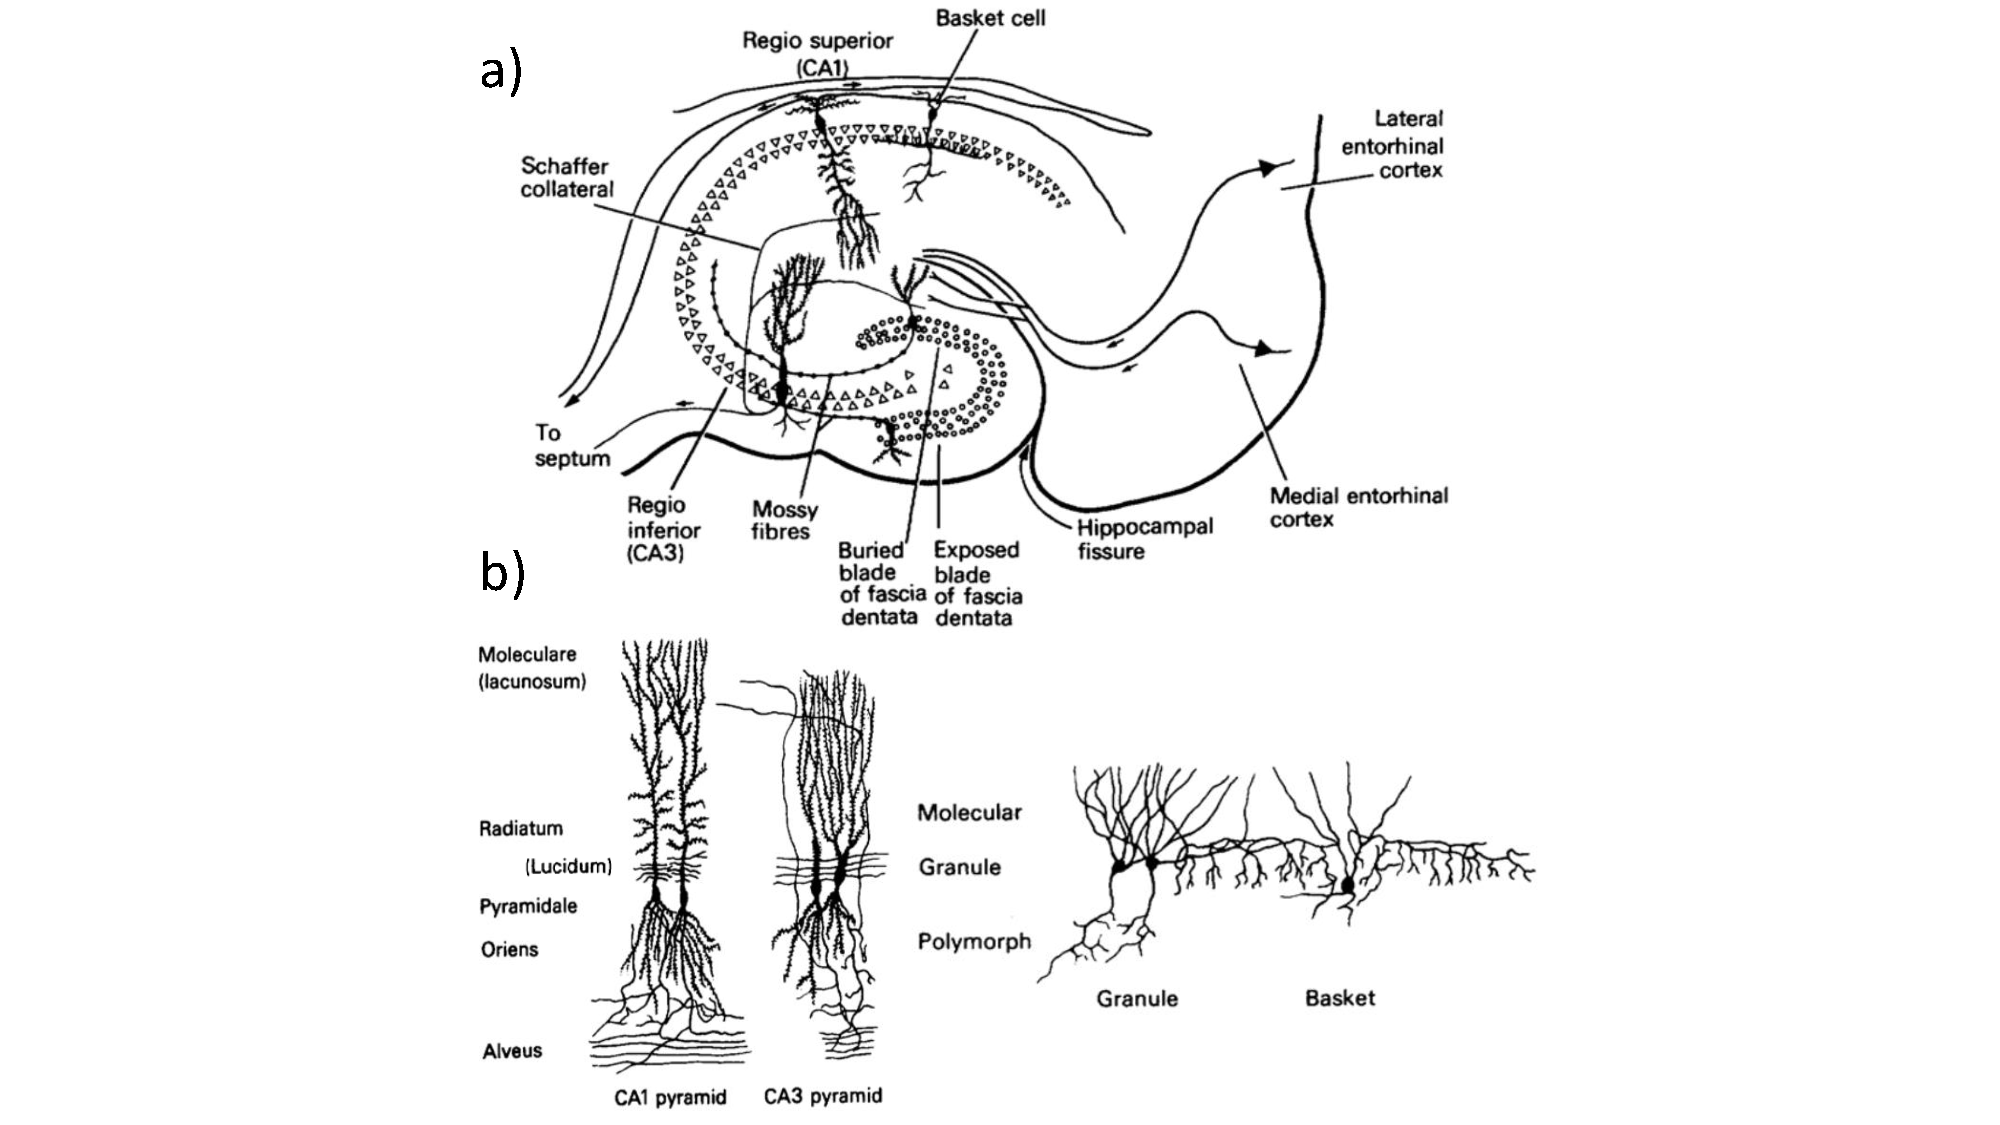
\includegraphics[trim={200 0 200 0},clip, width=\textwidth]{Figures/Chapter1/intro_fig_hipp_anat.pdf}
    \caption[Hippocampal anatomy.]{\textbf{Hippocampal anatomy.} A) Schematic representation of the mouse hippocampus and the connections between regions, adapted from [\cite{okeefebook}]. 
    B) Examples of CA1 and CA3 pyramidal cells (Cajal 1911, Figure 475) and dentate granule and basket cells [\cite{lorente1934}, Figure 10].}
    \label{fig:chap1:hippocampal_anat}
\end{figure}

% =========================================================== %
%      Subsection: Spatial information encoding cells         %
% =========================================================== %
\subsection{spatial information encoding neurons}
\label{chap1:sec:1:subsec2:spat_info_cells}
The main type of cells that conform to the cognitive map model was found by O’Keefe and Dostrovsky in 1971. 
Using electrophysiological recordings in the hippocampus, cells that fire predominantly in a specific location of a familiar environment (Figure \ref{fig:chap1:spatialnavigationcells}A) were observed.
These cells were called \textit{place cells}. 
Here, we will focus only on the main characteristics of place cells. 
We point to these fundamental reviews for an in-depth description of place cell function [\cite{moser2015place}; \cite{best2001spatial}].

\textbf{Place cells} are mainly found in the hippocampus proper, and their firing rate is modulated purely by spatial location; that is, they fire maximally when the animal's head is in a specific region of the environment (Figure \ref{fig:chap1:spatialnavigationcells}A). 
This region of the space is called the \textit{place field} of the cell (Figure \ref{fig:chap1:spatialnavigationcells}B).  
Here, we use the term environment in a generic way, but place cells have been mainly studied in constrained laboratory environments.
Interestingly, place cells have different characteristics, depending on the nature of the space that the animal explores.
In a two-dimensional space, such as the square/rectangular or circular boxes used in the early O'Keefe experiments [\cite{okeefe1976}], place cells fire at their place field location regardless of the direction of motion or speed of the animal.
However, in a one-dimensional environment (e.g., a linear track), place cells display a preferred direction of firing and fire much less, not at all or in a different location depending on the direction of motion on the linear track [\cite{mcnaughton1983}; \cite{okeefe1993}].
Place cells have also been found in three-dimensional environments, with three-dimensional place fields [\cite{yartsev2013}][\cite{grieves2020}].
The latter type of place cell has been observed in bats flying through a familiar environment [\cite{yartsev2013}] and, more recently, in rodents exploring three-dimensional environments [\cite{grieves2020}].

The way that place cells represent position is not limited to the firing rate but also involves the temporal aspect of their firing. 
Place cell firing is locked to the phase of the sinusoidal local field potential (LFP), which is called the theta rhythm, and hence to the population activity in the hippocampus [\cite{okeefe1993}].
The theta rhythm works as a sort of clock against which the network can measure time and temporally locate cell spikes, allowing place cells to identify locations in an environment with much finer precision than if only the rate code were used.
This is called \textit{temporal coding} [\cite{okeefe1993}; \cite{huxter2003}; \cite{buzsaki2004}; \cite{buzsaki2002}].

Neighboring place cells do not necessarily have similar or adjacent place fields. 
Furthermore, groups of anatomically close place cells typically have place fields that span the whole space, suggesting that place cells represent a complete and highly redundant representation of the environment [\cite{okeefe1976}; \cite{wilson1994}].
Once formed, these representations can be stable across days [\cite{hill1978}; \cite{muller1987}] or even weeks [\cite{thompson1990}].
However, not all place fields are stable, and plasticity of this neuronal representation of spatial information has been reported [\cite{mankin2015}; \cite{ziv2013}]. 
\begin{figure}
    \centering
    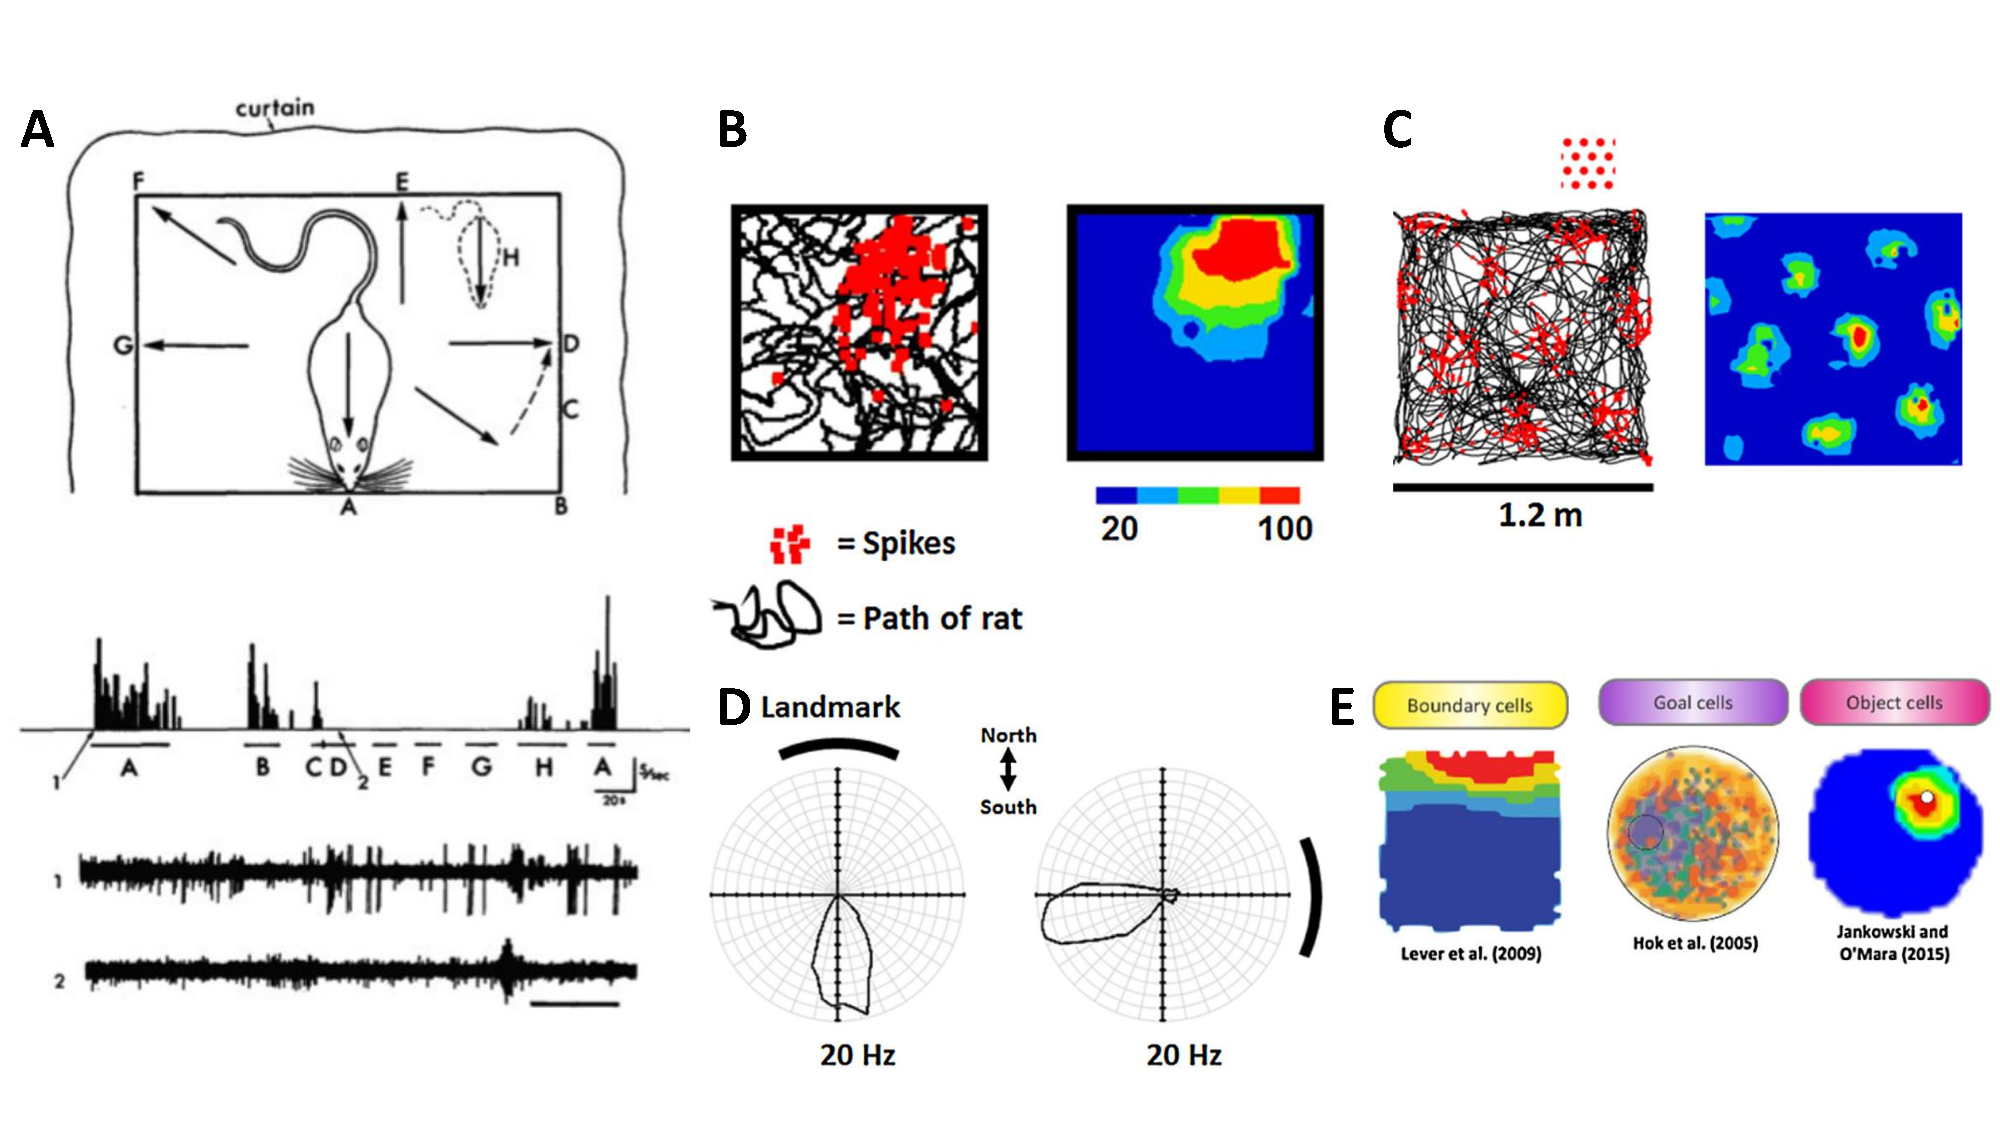
\includegraphics[width=\textwidth]{Figures/Chapter1/intro_fig_spatnav_cells.pdf}
    \caption[Spatial information-encoding cells]{\textbf{Spatial information-encoding cells.} 
    A) The first report of a place cell in the hippocampus of a freely moving rat. 
    The animal navigated a box (top). The cell fired only when the animal was in locations A and B. From O’Keefe and Dostrovsky (1971). 
    B) Spikes (red squares) from a single hippocampal cell and the path of the animal (black line) in a single trial (left). 
    On the right, the same data are shown as a heat plot of the dwell-time-adjusted firing rate (between peak and 20\% peak amplitudes), displaying the place field of the neuron. 
    C) Grid, close-packed hexagonal firing pattern of a single entorhinal grid cell. 
    Firing is depicted as in B). 
    Characteristic distances from the lattice are specific to each cell and relatively constant in different environments, suggesting the encoding of distances. 
    D) Two trials recorded from a postsubicular head direction cell in a symmetrical environment with a single polarizing landmark. 
    Polar plots show the firing rate as a function of the direction of the animal's head. 
    When the landmark is positioned north (left), the cell fires maximally when the animal's head faces south. 
    When the landmark is rotated to the east (right), the cell fires to the west, maintaining an equivalent relationship to the landmark. 
    This shows that cells are influenced by local cues and not by geocentric cues such as the Earth’s magnetic field. 
    B), C), and D) are adapted from \cite{grieves2017}. 
    E) Examples of other types of navigation cells; references are indicated in the figure.}
    \label{fig:chap1:spatialnavigationcells}
\end{figure}

How does this spatial representation arise in hippocampal cells based on the synaptic inputs that these cells receive? A large number of studies have focused on this question and provided important hints.
It is clear that visual information is important, as distal cues or landmarks surrounding the environment can influence place field formation [\cite{mullerkubie1987}; \cite{okeefe1978}; \cite{yoganarasimha2005}]. However, these inputs are not necessary. 
In fact, place cells fire in the same location in the dark in a familiar environment [\cite{save2000}; \cite{zhang2014}; \cite{markus1994}; \cite{quirk1990}], provided that other sensory cues are available, such as olfaction or tactility. 
These different sensory modalities are integrated outside of the hippocampus [\cite{jeffery2007}]. 
This indicates that place fields are higher order representations that integrate more primitive spatial constructs such as direction, self-motion, and boundaries. 
If sensory cues signal that the environment changes, a new and unique representation is formed in the hippocampal circuit [\cite{anderson2003}; \cite{okeefe1978}] in a process called remapping [\cite{mullerkubie1987}]. 
Importantly, in rats and mice, the animal must directly explore the physical space for place cells to form a spatial representation [\cite{rowland2011}]. 
In contrast, other mammals (e.g., primates) can form inferred allocentric representations of remote space if observed [\cite{rolls1999}; \cite{rolls1997}; \cite{rolls1995}]. 

To define a place cell and its place field, several criteria related to the firing rate, consistency of firing, and reliability have been used [\cite{okeefe1976}; \cite{thompson1990}; \cite{dombeck2010}]. 
Throughout this thesis, we will define a place cell as a cell in the hippocampus proper that carries a \textit{significant amount of information} about the animal's position in its firing activity (see also methods and later sections of the introduction for more details about the contextual definition of the word information).  

A key cell type in the spatial representation is \textbf{head direction cells} (Figure \ref{fig:chap1:spatialnavigationcells}D).  
Head direction cells are located in the presubiculum, and their firing is modulated by the facing direction of the head.
They were first found by Rank [\cite{ranck1984}; \cite{ranck1985}] and characterized in detail later [\cite{taube1990a.}; \cite{taube1990b}; \cite{taube1987}].
Here, by the term \textit{head direction}, we refer to the orientation of the head in the horizontal plane.
Head direction cells are similar in their characteristics to place cells. 
They have a preferred direction of firing that is independent of other behavioral factors. 
Each head direction cell has a different preferred direction. 
Preferred directions are equally distributed in the circle, meaning that there is no overall preferred direction of the network [\cite{taube1990b}].
Similar to place cells, the angular orientation of environmental cues is an important modulator of head direction cell activity (Figure \ref{fig:chap1:spatialnavigationcells}D) [\cite{goodridge1995}; \cite{taube1995a}; \cite{taube1990b}; \cite{zugaro2000}; \cite{knierim1995}] but is not necessary [\cite{mizumori1993}; \cite{yoder2011a}; \cite{yoder2011b}].
An interesting characteristic of head direction cells is that the angular relationship between preferred directions of different cells is preserved [\cite{skaggs1995}; \cite{yoganarasimha2005}].
Hence, when remapping of the environment occurs in which one cell changes its orientation, the rest of the cells coherently change their functional properties [\cite{skaggs1995}; \cite{yoganarasimha2005}].

With the information encoded in place cells and head direction cells, the cognitive map model can build positions and measure angles. 
However, another crucial requirement for the map to be completed is a way of measuring distances, i.e. to establish the metric of the map.
In 2005, a cell type that could achieve this task was identified in the Moser's lab: \textbf{grid cells}. 
Grid cells are cells that fire in multiple discrete and regularly spaced locations. 
Grid cells form a triangular or, equivalently, a hexagonal lattice (Figure \ref{fig:chap1:spatialnavigationcells}C). 
These cells are found in the medial entorhinal cortex (mEC), in the postrhinal cortex [\cite{fyhn2004}; \cite{hafting2005}; \cite{fyhn2008}] and in the pre- and para-subiculum [\cite{boccara2010}]. 

Grid cells share some characteristics with place cells and head direction cells.
Their pattern of firing arises in familiar environments and partially relies on distal visual cues [\cite{hafting2005}]. 
If environmental cues rotate, grid patterns consistently do so too [\cite{hafting2005}]. 
Deformation of the environment causes deformation of the grid patterns [\cite{barry2007}; \cite{stensola2012}].
Similar to head direction cells, the angles and distances between grid patterns of different grid cells are preserved, and when the environment rotates or moves, the patterns adapt in a coherent fashion, maintaining a stable relationship [\cite{fyhn2007}] across grid cells.
This suggests that grid cells work cooperatively, as an interconnected matrix known as an attractor network [\cite{mcNaughton2006}].
Moreover, the spacing between peaks of grid patterns varies as a function of location in the entorhinal cortex. 
The scales of the patterns increase in discrete jumps from the dorsal to ventral sides of the entorhinal cortex [\cite{brun2008}].
Each animal can display 3 or 4 different scales[\cite{brun2008}]. 

An additional functional class of cells that contain spatial information about the outer environment is \textbf{boundary cells} (Figure \ref{fig:chap1:spatialnavigationcells}E left).
Boundary cells, or boundary vector cells, are located in the subiculum and selectively respond to environmental boundaries. 
Boundaries can be walls, low ridges, and vertical drops. The color, texture, and odor of these boundaries do not seem to influence the firing of boundary cells [\cite{lever2009}].
Interestingly, the existence of boundary cells was first hypothesized to explain the observation that after elongating one side of a rectangular box, place fields stretched accordingly [\cite{oKeefe1996}].
This led researchers to hypothesize the existence of cells that fire in relation to environmental boundaries and that place cell firing could arise as a thresholded sum of a subpopulation of such neurons [\cite{barry2006}; \cite{burgess1997}; \cite{hartley2000}]. 
Cells that partly fit this theoretical description were later found in several regions of the brain, including the subiculum [\cite{barry2006}], presubiculum and parasubiculum [\cite{boccara2010}], medial entorhinal cortex [\cite{bjerknes2014}; \cite{savelli2008}; \cite{solstad2008}], anterior claustrum [\cite{jankowskiomara2015}], and rostral thalamus [\cite{jankowski2015}].

In a more formal definition, boundary vector cells can be defined as neurons that $i)$ fire when the animal encounters an environmental boundary in its preferred direction, and $ii)$ their firing is driven by the memory of the boundary's position relative to the animal, based not only on perceptual cues but also on self-motion information [\cite{lever2009}; \cite{raudies2012}; \cite{raudieshasselmo2012}]. 
Notably, boundary cells fire at a specific distance from the boundary, and this distance is different for boundary cells in different brain regions [\cite{bjerknes2014}; \cite{solstad2008}; \cite{jankowski2015}; \cite{lever2009}].

Altogether, place cells, head direction cells, grid cells, and boundary vector cells lie at the core of the cognitive map model and are the most relevant and studied type of cells in the context of spatial navigation. 
This obviously does not imply that other types of spatially informative cells might not be present; therefore, there is room for more \textit{types} of these cells to be discovered in future investigations. 
In particular, cells in which the firing activity is modulated by more abstract or complex information have been described, including \textbf{object cells}, \textbf{goal cells}, \textbf{boundary-off cells}, \textbf{perimeter cells}, and \textbf{band cells}, among others (Figure \ref{fig:chap1:spatialnavigationcells}E center and right). 

What is the relation between the firing patterns of all these functional classes of cells?
Mathematically, it can be shown that place cells can be formed by summing two grids with different spacings or, equivalently, by summing two border cells. Similarly, it has been demonstrated that grid cells can be built by combining the activity of band cells. 
However, a complete understanding of the function and implication of each of these functional classes of cells and their interactions in contributing to spatial navigation has not yet been achieved. 
Moreover, as mentioned earlier, the functional classes listed above could be only the tip of the iceberg. 
The more the extended hippocampal formation is studied, the larger the number of new cell classes that are described will be. 

% =========================================================== %
%      Subsection: Calcium as a proxy of spiking activity     %
% =========================================================== %
\subsection{Calcium as a proxy of spiking activity}
\label{chap1:sec:1:subsec3:calcium_proxy_spikes}
With a few exceptions, the large majority of the research presented in the previous sections has relied on electrophysiological recordings of neuronal activity.  
Electrophysiology has long been the preferred technique by which to interrogate brain activity, mostly because of its versatility, high signal-to-noise ratio, high temporal resolution, and ability to capture a large spectrum of neuronal signals, from individual action potentials (AP) and subthreshold membrane potential to network oscillations [\cite{buzsaki2012}][\cite{margrie2003}][\cite{hubel1959}].
In the last few decades, huge technological improvements in micro- and nanofabrication techniques for multielectrode arrays [\cite{bareketkeren2012},\cite{spira2013},\cite{viventi2012},\cite{jun2017}] have helped improve the yield, sampling density, and biocompatibility of electrical probes.
At the same time, the development of modern analytical methods has permitted the extraction of many types of information from this kind of recording [\cite{agarwal2014}; \cite{sheinidelson2017}]. 
Although electrophysiologial approaches have come a long way and are a reliable and versatile way of studying neuronal activity, they also suffer from limitations. 
For example, in unit recordings, they are biased towards the detection of cells with high firing rate; at the microcircuit level, they allow limited structure-function correlations [\cite{dombeck2010}], and importantly, they poorly discriminate between genetically selected neuronal populations. 
Moreover, electrophysiological recordings are blind to the form of excitability that does not generate electrical signals, such as the calcium excitability of certain glial cells.
Alternative experimental methods partially overcome some of these limitations. 
In the last 3 decades, optical imaging methods and fluorescent activity reporters have provided an additional and efficient tool with which to study neural networks and their functions, overcoming some of the limitations of the methods described above [\cite{ohki2005},\cite{shoham1999}; \cite{grienberger2012}; \cite{bovetti2014}; \cite{yang2017}]. 
The current success of these optical methods relies on two main technical advances: the synthesis of fluorescent calcium indicators and the development of nonlinear microscopy. 
The latter technique made it possible to record large ensembles of neurons (up to 10.000) at subcellular spatial resolution in the intact brain [\cite{bovetti2014}; \cite{yang2017}; \cite{svoboda2006}].

Action potential firing, as well as strong synaptic inputs, leads to the opening of voltage-gated calcium channels in neurons, which induces transient elevations in cytoplasmic $Ca^{2+}$ concentration.
These variations are typically in the range of 50-100 $nM$ to 5-10 $\mu M$ and can be detected by fluorescence calcium indicators.
In this approach, neurons stained with these fluorescent compounds change the fluorescence emitted from the somatic region upon AP firing [\cite{yuste1991}].
Calcium transients decay over 100–500 $ms$ through diffusion, the activity of calcium extrusion mechanisms, and internal buffering processes [\cite{grienberger2012}].
Importantly, cells that are not electrically excitable may display intracellular calcium transients. 
This is the case, as seen in the next section (\ref{chap1:sec:2:subsec2:astro_calcium_signals}), for glial cells, particularly astrocytes.
Astrocytes display variations in their intracellular calcium levels that correlate with neuronal activity.  
  
The first calcium indicators developed were synthetic [\cite{grienberger2012}; \cite{tsien1981}]. 
These dyes typically have high signal-to-noise ratio [\cite{stosiek2003}], [\cite{grienberger2012}], [\cite{wiederschain2011}], [\cite{helmchen2002}]; however, they do not easily allow labeling of genetically identified cell populations.
An important breakthrough in overcoming this limitation was developed by the laboratory of the Nobel Prize winner Roger Tsien [\cite{miyawaki1997}] who developed the first versions of protein-based genetically encoded calcium indicators (GECIs). 

By combining these fluorescent calcium binding proteins with cell-type specific promoters, subcellular targeting sequences, and transgenic technology, stable expression in distinct cell subpopulations (Figure \ref{fig:chap1:astro_calcium}) over prolonged periods of time is possible [\cite{grienberger2012}; \cite{knopfel2006}; \cite{looger2012}; \cite{chen2013}]. 
The applications of GECIs were initially restricted due to their limited signal-to-noise ratios and slow response kinetics [\cite{ohkura2005}; \cite{tallini2006}; \cite{tian2009}]. 
However, incredible progress in the development and refinement of brighter and more sensitive variants has been achieved during the last 15 years, and newer GECIs rival synthetic calcium indicators in many respects [\cite{horikawa2010}; \cite{palmer2011}; \cite{akerboom2012}]. 
For example, ultrasensitive genetically encoded calcium indicators of the GCaMP6, GCaMP7 family [\cite{chen2013}; \cite{dana2019}] and RCaMP family [\cite{akerboom2013}; \cite{dana2016}; \cite{ohkura2012}; \cite{forli2018}] can report, under optimized experimental conditions, the calcium transients associated with the discharge of a single AP in vivo.
% =========================================================== %
%           Subsection: 2-photon calcium imaging              %
% =========================================================== %
\subsection{2-photon calcium imaging}
\label{chap1:sec:1:subsec4:2_photon_imaging}

The design, development, and optimization of fluorescent activity indicators opened the door to a wide range of possibilities and demonstrated that it was possible to monitor neural activity indirectly by capturing changes in the intracellular concentrations of certain ions. 
However, fundamental advances in \textbf{optical imaging} are also needed for the application of fluorescent calcium indicators to the study of neural or glial network function in the intact CNS [\cite{grienberger2012}; \cite{bovetti2014}; \cite{yang2017}].
One of these fundamental advances is multiphoton microscopy-in particular, two-photon laser-scanning microscopy (2PLSM).
2PLSM saw its first experimental validation approximately 30 years ago, and since then, it has revolutionized biological imaging due to its unprecedented combination of high resolution and high contrast, even when imaging hundreds of microns deep inside intact tissue [\cite{denk1994}], [\cite{helmchen2005}].
Briefly, 2PLSM is a laser-scanning method that exploits localized ‘nonlinear’ excitation to stimulate fluorophores only within the thin raster-scanned plane [\cite{zipfel2003}]. 
Two-photon (2P) fluorophore excitation was first conceived by Marie Goeppert-Mayer [\cite{goppertmayer1931}] and relies on the idea that when two photons arrive \enquote{quasi-simultaneously}, that is, within fractions of a $fs$, at the fluorophore, their energy is absorbed to promote the transition of one electron of the fluorophore from the ground state to the excited state.
The electron in the excited state then decays following the normal fluorescence-emission pathway, as in single-photon fluorescence excitation (Figure \ref{fig:chap1:optical_imaging}A) [\cite{pawley2006}].
In this process, fluorophore excitation relies on higher-order light-matter interactions, thus having a nonlinear dependency on the incident light intensity [\cite{svoboda2006}], [\cite{helmchen2005}]. 
2PLSM represents an improvement with respect to standard wide-field fluorescence, wherein excitation is due to the absorption of a single photon and therefore depends linearly on the light intensity. 
\begin{figure}
    \centering
    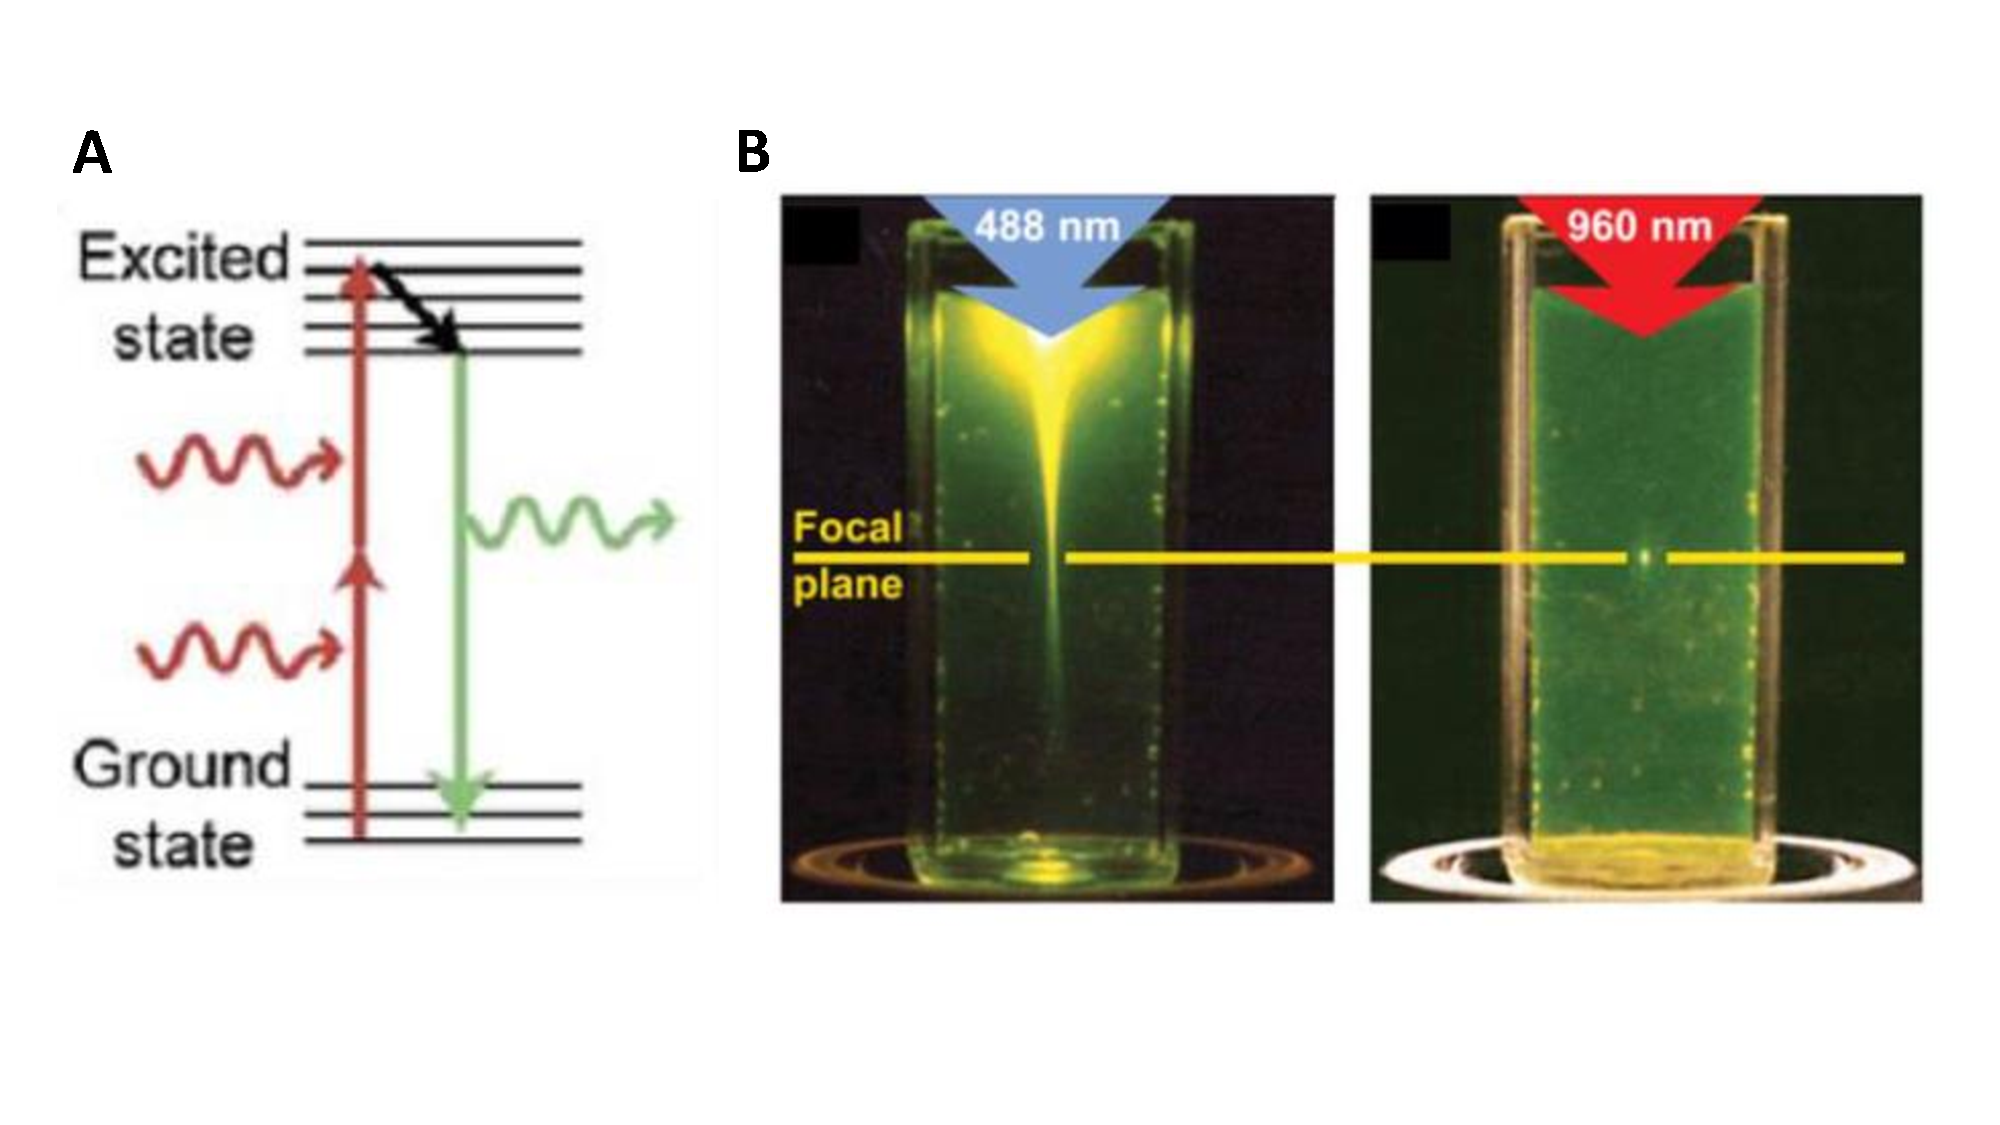
\includegraphics[trim={0 90 0 0},clip, width=\textwidth]{Figures/Chapter1/intro_fig_optical_imaging.pdf}
    \caption[Two-photon excitation of fluorescent molecules.]{\textbf{Two-photon excitation of fluorescent molecules.} 
    A) Simplified Jablonski diagram of the two-photon emission process. Adapted from \cite{svoboda2006}. 
    B) Experimental demonstration of the localization of excitation in 2P imaging using focused (0.16 NA) $fs$ pulses of $960\ nm$ light (right) in comparison to single-photon excitation of fluorescein by focused $488\ nm$ light (0.16 NA) (left). 
    Adapted from \cite{zipfel2003}.}
    \label{fig:chap1:optical_imaging}
\end{figure}

Three characteristics of 2P microscopy provide a comparative advantage with respect to other approaches when imaging thick samples in vivo [\cite{helmchen2005}]: 
\begin{enumerate}
    \item \textbf{Imaging depth and phototoxicity}: 2P absorption in commonly used fluorophores occurs in the near-infrared wavelength range ($700$-$1100 nm$). 
    This wavelength range is generally less phototoxic and penetrates deeper into scattering tissue compared to visible light.
    \item \textbf{High resolution}: The fluorescence signal (S) depends on the square of the light intensity ($S\ \alpha \ I^2$). Thus, when focusing the laser beam through a high NA objective, 2P absorption under unsaturated conditions is limited to the perifocal region (Figure \ref{fig:chap1:optical_imaging}B) [\cite{nagy2005}].
    \item \textbf{No pixel cross-talk}: Because the sample is sequentially excited, meaning that the signals are collected point-by-point, the pixel cross-talk observed in wide-field imaging is virtually absent.
\end{enumerate}

Since the first validation of 2PLSM [\cite{denk1990}], several advancements have been made in several aspects, leading to higher signal-to-noise ratios, better temporal resolutions, and larger field-of-view dimensions, penetration depths and accessible volumes for in vivo imaging (reviewed in \cite{yang2017}). 
Combining 2PLSM with fluorescent activity reporters constitutes one of the most powerful approaches to investigating neuronal networks in the intact CNS at cellular resolution over $mm$ of brain tissue.
 
Thanks to its unique advantages, researchers in the spatial navigation field have increasingly used 2P calcium imaging for the interrogation of hippocampal circuits [\cite{gauthier2018}; \cite{rubin2015}; \cite{dombeck2010}].
Together with appropriate analytical tools [\cite{sheintuch2017}], these approaches allow the study of anatomically and genetically identifiable ensembles of cells across days in awake, behaving animals, opening the door the a whole range of new investigations that wold not be possible otherwise. 

All the aforementioned research has focused only on neuronal networks. 
However, neurons represent approximately half of the cells in the mammalian brain. 
The main nonneuronal population of cells in the mammalian brain is called \textbf{glial cells}.
Although glial cells do not have electrical activity similar to neurons, they express rich intracellular calcium dynamics and interact with neuronal cells in active ways. 
In this thesis, we will approach the question of whether glial cells play a role in spatial navigation in the mouse brain and what that role may be. 

We will briefly describe the types of glial cells that can be found in the brain, focusing on a particular subtype, \textbf{astrocytes}, their characteristics and their role in modulating neuronal activity. 
% =========================================================== %
%                      Section: Glia                          %
% =========================================================== %
\section{Glia}
\label{chap1:sec2:glia}
Glial cells were first observed as early as the mid 19th century by Virchow [Virchow, 1856], and were better described and brought to wider attention by Santiago Ram{\'o}n y Cajal and P{\'i}o del R{\'i}o Hortega a few decades later thanks to the development of the chloride-sublimate technique, which is a staining technique that specifically targets astrocytes [\cite{cajal1895}; \cite{delriohortega1921}].
At this time, glial cells were thought to play a strictly structural role in the brain.
If anything, the terminology used to describe them would be sufficient to understand the hypothesized role—glial cells were described as \textit{Zwishchenmass}, which is German for \textit{in between mass}; \textit{Nervenkitt}, or \textit{nerve glue} in English; and finally, the current terminology \textit{glial cell} comes from the Greek word \textit{gl\'ia}, meaning \textit{glue}.
It was not until the second half of the 20th century when electrophysiological characterizations and physiological studies of glial cells permitted the understanding of the wide range of vital functions that glial cells have in the functioning of the central nervous system [\cite{morrison1981growth}; \cite{bowman1984}; \cite{kettenmann1984}; \cite{kettenmann1984aspartate}; \cite{cornell-bell1990}; \cite{araque1998}; \cite{bezzi1998prostaglandins}]. 
Phylogenic studies show that all organisms with a central nervous system have glial cells, and interestingly, the ratio of astrocytes to neurons is different depending on the animal species and on the brain region, with intriguing correlations with the brain complexity and neuronal density [\cite{herculano2011scaling}; \cite{herculano2014}].   
Throughout evolution, glial cells have diverged into specialized subgroups with different characteristics and functions. 
In mammals, glia can be divided into two large groups based on their size: \textbf{microglia} and \textbf{macroglia}.
Macroglia can be further subdivided into three major groups: \textbf{oligodendrocytes}, \textbf{NG2-positive cells}, and \textbf{astrocytes}. 

Unlike the rest of the glial cells, \textbf{microglia} originate from yolk-sac progenitors that only populate the brain during development (reviewed in \cite{kim2005microglia}; \cite{kettenmann2011physiology}).
They represent the main immunocompetent and phagocytic cells of the central nervous system [\cite{filiano2015interactions}] and cover a major part of the adult brain in individual nonoverlapping domains.
Microglia sense the environment through the movement of their filopodia, which rapidly reacts to abnormalities or damage [\cite{nimmerjahn2005resting}; \cite{cronk2013microglia}].
In adition to the immune role, microglia have recently been hypothesized to have an active role in the healthy brain. 
Opinions on this matter are, however, controversial. 
Some studies show that microglia could be involved in motor-dependent synapse formation [\cite{parkhurst2013microglia}] and in features as high-order as learning or social behavior [\cite{torres2016dynamic}; \cite{kierdorf2017microglia}], while others have shown that ablation of microglia barely produces any alterations or pathologies in healthy adult mice [\cite{elmore2014colony}; \cite{elmore2015characterizing}; \cite{bruttger2015genetic}].
When comparing the results of these studies, it should be considered that these discrepancies might be due to the major methodological differences in those studies [\cite{jakel2017glial}].

\textbf{Oligodendrocytes} are large macroglial cells that were first observed by Pío del Río Hortega in the first half of the 20th century. 
Their function is to insulate axons with self-produced myelin to allow fast saltatory conduction and provide trophic support to axons [\cite{nave2010myelination}].
However, oligodendrocytes have also been found in sparsely myelinated brain regions, and presumably, nonmyelinating oligodendrocytes might have other overlooked functions.

The more recently discovered \textbf{NG2-positive cells} are oligodendrocyte precursors [\cite{raff1986proliferating}].
Their first evident function is to form and maintain a homeostatic network, preserving stable cell numbers stable by generating mature myelinating oligodendrocytes throughout their lifetime [\cite{dimou2008progeny}; \cite{rivers2008pdgfra}; \cite{psachoulia2009cell}; \cite{simon2011progenitors}; \cite{hughes2013oligodendrocyte}] under physiological conditions.
NG2-positive cells form functional synapses with neurons.
An associated phenomenon was first observed in the hippocampus [\cite{bergles2000glutamatergic}] but later described in other brain regions [\cite{karadottir2005nmda}; reviewed in \cite{sun2013synaptic}].
Such synapses are uniderectional in the sense that they can only receive neuronal signals but cannot generate action potentials on their own and further propagate them [\cite{de2010excitability}]. 
This shows that NG2-positive cells can accurately sense synaptic activity and suggests that this process may modulate their functions.

The last large group of glial cells in the brain is \textbf{astrocytes}.
As mentioned before, astrocytes and their intracellular calcium signals are a key aspect of this thesis work. 
For this reason, within the next few sections, we will focus on their function, anatomy and known relationship with neuronal activity. 

% =========================================================== %
%                    Subsection: Astrocytes                   %
% =========================================================== %
\subsection{Astrocytes}
\label{chap1:sec:2:subsec1:astrocytes}
Astrocytes are the most abundant type of glial cell in the mammalian brain [\cite{herculano2014}].
Despite being one of the first glial cells discovered approximately 150 years ago, their description and the understanding of their role in brain function are still far from complete.
Astrocytes do not represent a single homogeneous cell type and can be subdivided into several types depending on their morphology, molecular profile or function [\cite{batiuk2020}]. 

From a morphological point of view, astrocytes can be roughly divided into two types: \textbf{fibrous} and \textbf{protoplasmic}.
The first is a star-shaped cell with regular contours present mainly in the white matter of the brain and spinal cord and in the optic nerve and the retina fiber layer.
Fibrous astrocytes are characterized by their elongated morphology, with long processes running parallel to the axon bundles that make contact with myelinated axons and with oligodendrocytes.
They have fewer processes than protoplasmic astrocytes.
Their processes spatially overlap in their domains and extend to perivascular, subpial, and axonal endfeet [\cite{lundgaard2014white}].

Protoplasmic astrocytes, on the other hand, have a “bushy” and irregular morphology, with a small round somata of $\sim 10 \mu m$ in diameter (Figure \ref{fig:chap1:astro_anatomy_cajal}). 
They present $5-10$ primary processes that further branch into thousands of branchlets and leaflets to form dense arborizations that contact neurons at synapses [\cite{bushong2002}]. 
Astrocytic processes also end in large endfeet that contact the vasculature [\cite{nagelhus2013}; \cite{verkhratsky2015}] (schematically represented in Figure \ref{fig:chap1:astro_anatomy_cajal}). 
Unlike fibrous astrocytes, protoplasmic astrocytes mainly populate the gray matter in the brain and have domains with well-defined borders that minimally overlap with each other [\cite{bushong2002}].
A single astrocyte arborization can cover 20,000 to 80,000 $\mu m^3$, contacting 300 to 600 dendrites and potentially 100,000 individual synapses [\cite{bushong2002}; \cite{halassa2007}].
This dense connectivity allows astrocytes to control several processes, including ion homeostasis, neurotransmitter clearance, trophic support to neurons, and neuromodulation.
Interestingly, astrocytic domain boundaries have been proposed to be functional units [\cite{perea2014}; \cite{fellin2009}].
For example, astrocytes could play the role of controlling and modulating \textit{functional islands} formed by synapses confined within the area of influence of a single astrocyte (Figure \ref{fig:chap1:astro_neuro_modulation}C) [\cite{halassa2007}; \cite{fellin2009}].
Indirect support for this hypothesis comes from the observation that branching and position processes are dynamic [\cite{kacerovsky2016stargazing}], strongly dependent on neuronal activity [\cite{genoud2006plasticity}], and brain region-dependent [\cite{chai2017}].   
For example, when comparing striatal and hippocampal astroglial populations, it was noted that despite having the same somatic volume, equivalent number of primary branches, and total cell volume, hippocampal astrocyte territories are more constrained and display a tighter physical interaction with excitatory synapses [\cite{chai2017}] compared to striatal territories.

If astrocytes are so closely related to neuronal function and, as said before, have large and dense areas of influence, what are astrocyte's functions in the brain? 
This question still represents a very active area of research. 
Here, we will enumerate some of the known functions that have been ascribed to astrocytes. 

Astrocytes are involved in the \textbf{control of cerebral blood flow} through \textbf{gliovascular coupling}.
Matching the blood flow to the neuronal metabolic needs is crucial for healthy brain functioning, which is achieved by astrocytes in a twofold manner. 
First, by regulating the dilation of blood vessels, it has been proven that synaptic activity mediates cytoplasmic calcium increases in astrocytes, which, in turn, promote the dilation of neighboring arterioles [\cite{zonta2003}; \cite{attwell2010}].
At the same time, astrocytes regulate vasoconstriction through the release of 20-hydroxyeicosatetraenoic acid (20-HETE) [\cite{metea2006}; \cite{attwell2010}].
Interestingly, astrocytes seem to \textit{decide} drive dilation or constriction based on local oxygen levels and metabolic states [\cite{macvicar2015}]. 
\begin{figure}
    \centering
    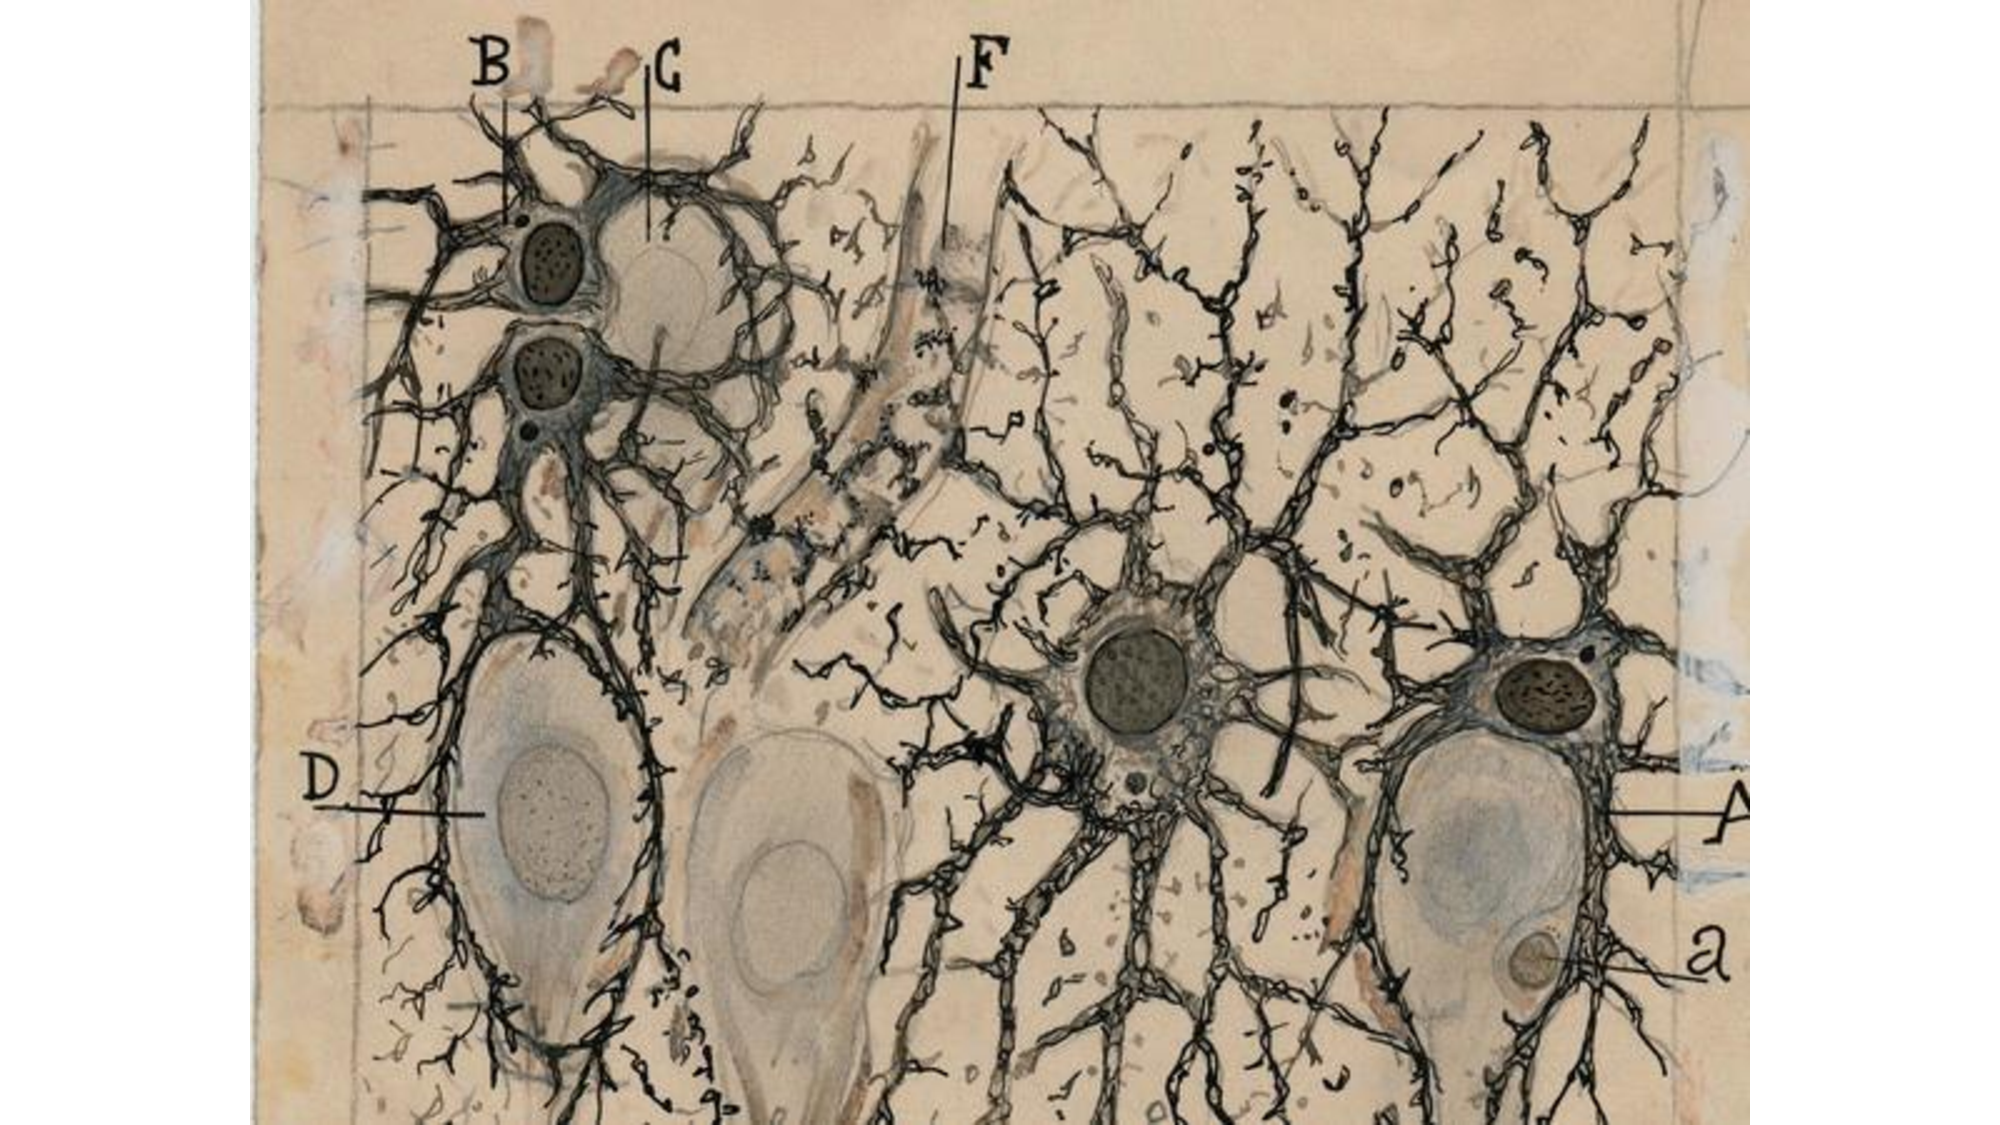
\includegraphics[width=\textwidth]{Figures/Chapter1/intro_fig_astro_cajal.pdf}
    \caption[Cajal's drawing of astrocytes]{\textbf{One of Cajal's original drawings of astrocytes in the hippocampus of a man three hours after death.} This beautiful representation exemplifies several of the properties of astrocytes discussed herein. Note the connections with blood vessels, the small overlapping areas of domains, the somas, the large and distal processes and how astrocytic processes surround neuronal cell bodies.
    Adapted from \cite{swanson2017beautiful}}
    \label{fig:chap1:astro_anatomy_cajal}
\end{figure}

Given the enormous energy consumption in the brain, the regulation of oxygen and glucose availability must be tightly controlled.
This is, of course, in part regulated by blood flow. 
However, while oxygen freely diffuses in the brain, glucose and other metabolites need specialized transporters to travel through cell membranes.
The need for energy depends on neuronal activity, which can go from completely silent to a high firing rate in milliseconds, in turn demanding up to a 30-fold increase in metabolic consumption [\cite{attwell2001}]. 
It has been demonstrated that astrocytes, which are in contact with both blood vessels and synapses, strongly and tightly control active \textbf{metabolic support} to neurons. 
This can be achieved through a variety of processes that are still the subject of intense research. 
Glucose is preferentially taken up by astrocytes rather than neurons [\cite{pellerin2007}]. 
Within astrocytes glucose enters glycolysis, producing lactate.
Lactate is then delivered to neurons via the astrocyte-neuron lactate shuttle (ANLS) [\cite{pellerin1994}]. 
Thus, astrocytes are involved in the metabolic support of neurons not only through blood flow regulation but also through direct delivery of energy substrates. 

Astrocytes, together with microglia, have a key role in the \textbf{immune response} of the brain under both physiological and pathological conditions.
Upon brain injury or disease, astrocytes become reactive, drastically changing gene expressions [\cite{zamanian2012}].
These changes induce morphological and functional alterations that lead astrocytes to enter one of two distinct reactivity profiles, depending on the nature of the insult. 
Inflammatory insult leads astrocytes to enter what has been called \textit{A1}, which is a reactivity profile leading to synapse pruning.
On the other hand, ischemic injury leads to activation of reactivity profile \textit{A2}, which is responsible for the growth and survival of neurons and synapses. 
These contrasting mechanisms coexisting in the same cell type prove once more the complexity and diversity of astrocytic function. 
Moreover, under physiological conditions, astrocytes continue to play a role in immune protection of the brain by controlling the functionality of the blood-brain barrier (BBB)[\cite{almutairi2016factors}]. 
Interestingly, astrocytes have been shown to be involved in BBB formation during development [\cite{hayashi1997}]. 

In addition to the aforementioned functions, astrocytes play key roles in ionic [\cite{sibille2014}; \cite{nwaobi2016}], water [\cite{nielsen1997}; \cite{risher2009}] and neurotransmitter [\cite{danbolt2001glutamate}; \cite{herman2007}] homeostasis. 
Astrocytes can rapidly change their volume and intercellular communicative capacity, which allows them to redistribute water across astrocytic networks.  
They can redistribute $K^+$ ions through $K^+$ spatial buffering and are the only cells in the central nervous system that can synthesize glutamate and GABA from glucose. 
Astrocytes are thus an incredibly versatile and complex cell in the brain. A key aspect of astrocyte physiology is their excitability based on intracellular calcium signals and the relation of this process to neuronal function. 
We will discuss these aspects in the next sections. 

% =========================================================== %
%        Subsection: Calcium signaling in astrocytes          %
% =========================================================== %
\subsection{Calcium signaling in astrocytes}
\label{chap1:sec:2:subsec2:astro_calcium_signals}
% As inexpert scientists, we PhD students have a bias view of the way research works towards positive discoveries and confirmed hypothesis. 
% Simply because our biggest source of information are publications, and the chances of getting a story published that states \enquote{we formulated \textbf{this} hypothesis, and found it to be wrong} are very low, there's a lack of charm in failure that prevents unsuccessful hypothesis to be known. 
% Which is regrettable, because proven wrong hypothesis are at least as informative as positive results.
% With brilliant examples like the Michelson-Morley experiment in 1887, where the two physicist trying to prove the existence of the aether, the medium in which light was thought to propagate, proved instead that it didn't exist.  
% And in the way invented the interferometer. 
% Invention that was later crucial for the development of the special theory of relativity and, more recently, for the detection of gravitational waves.
% We can go even further and say that logic allow us \textit{only} to falsify theories, but, on the other hand, to prove a theory \textit{correct} is impossible. 
% We can get encouraging results, experiments that help us gain confidence in our working hypothesis, but not really prove it.
% On the other hand, one counterexample is all that is needed to prove it wrong.
% As Einstein eloquently put it: 

% \begin{quote}
% \textit{The scientific theorist is not to be envied. For Nature, or more precisely experiment, is an inexorable and not very friendly judge of his work. It never says \enquote{Yes} to a theory. In the most favorable cases it says \enquote{Maybe}, and in the great majority of cases simply \enquote{No}. If an experiment agrees with a theory it means for the latter \enquote{Maybe}, and if it does not agree it means \enquote{No}. Probably every theory will someday experience its \enquote{No} —most theories, soon after conception.}
% [Albert Einstein: the human side: New glimpses from his archives. Dukas and Hoffman 1922]
% \end{quote}
% Perhaps a way to compensate for this bias is to get rid of the miss-conception that falsifying an hypothesis represent failure but instead call it for what it is, a scientific discovery.  

% In a way, a fruitful, but less interesting substitute of self-falsified hypothesis are the stories of scientist trying to prove \textit{other} peoples theories wrong, because controversy, unlike failure, sells journals.
% One of the highly interesting and still active controversies in neuroscience is the question whether calcium concentration elevations in astrocytes regulates neuronal and vascular function.
% This has led in the last few decades to a series of works by different groups that appeared to be contradictory, and different research lines have been seemingly proving each other wrong to give rise to a better and more profound understanding of the subject.  
% We will not refer here the complete story that has been brilliantly summarized by Bazargani and Attwell [Bazargani and Attwell 2016], but will refer only some characteristics of calcium signaling in astrocytes that are relevant for the understanding of this work.

Astrocytes, unlike neurons, are electrically nonexcitable cells.
However, astrocytes display changes in the intracellular concentration of calcium ions and $Ca^{2+}$ fluctuations have been considered the main form of excitability for this type of glial cell.
An extensive amount of work in the last few decades has been dedicated to understanding the origin of $Ca^{2+}$ transients, as well as whether these fluctuations are somehow relevant for neuronal regulation, and if so, how.
To date, many of these questions remain largely unanswered. 
However, increasing evidence points to calcium signaling in astrocytes being involved in several processes [\cite{araque2014gliotransmitters}; \cite{volterra2014astrocyte}; \cite{khakh2019emerging}]. 
\begin{figure}[h]
    \centering
    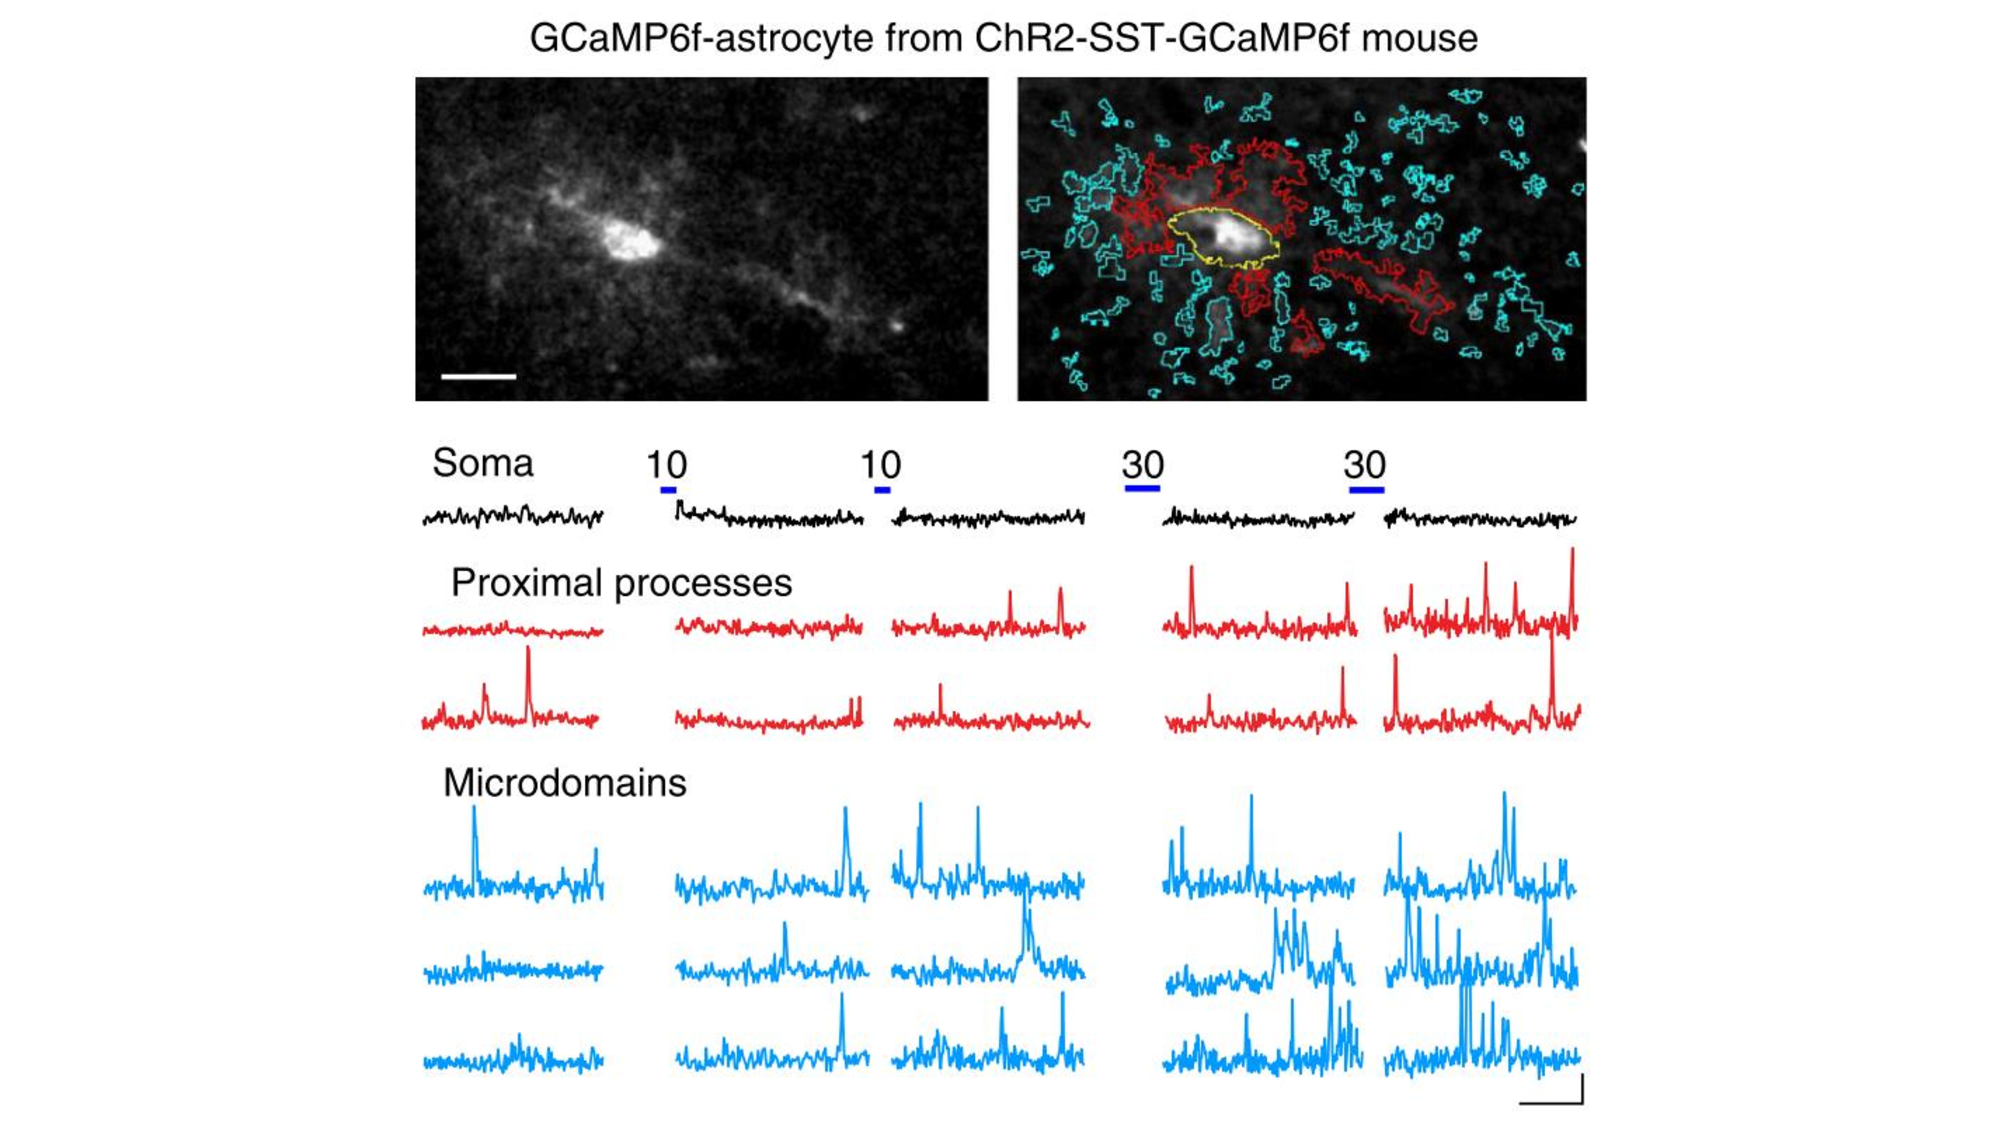
\includegraphics[trim={200 0 200 0},clip,width=\textwidth]{Figures/Chapter1/intro_fig_astro_calcium.pdf}
    \caption[Astrocytes present complex calcium transients in their somas and processes.]{\textbf{Astrocytes present complex calcium transients in their somas and processes.} 
    Image of GCaMP6f astrocytes in layer 2/3 SSCx from an adult ChR2-SST-GCaMP6f mouse that underwent SST interneuron optogenetic stimulation. 
    ROIs are depicted for the soma (yellow), proximal processes (red) and more distal processes (blue); scale bar, is 20 $\mu m$ (top). 
    Calcium signal dynamics in example compartments show the difference between transients depending on the region of the astrocyte; scale bars are $50\ s$, $20\% \frac{dF}{F0}$. Adapted from \cite{mariotti2018}.}
    \label{fig:chap1:astro_calcium}
\end{figure}

Baseline levels of $Ca^{2+}$ in astrocytes are higher than those in neurons, and this concentration varies inside each cell, being higher in processes than in the soma [\cite{zheng2015}].
This already indicates its within-cell complexity (Figure \ref{fig:chap1:astro_calcium}). 
In astrocytes, $Ca^{2+}$ fluctuations can have different sources, the first of which is intrinsic. 
In fact, $65\%$ of astrocytes in hippocampal slices exhibit asynchronous and localized $Ca^{2+}$ transients, even in the absence of neuronal activity [\cite{nett2002}; \cite{hirase2004}].
The role and relevance of these untriggered events are still largely undefined. 

In addition to spontaneously, calcium signals in astrocytes can also be triggered by neurotransmitter release through the activation of mostly metabotropic receptors for neurotransmitters.
For example, glutamate has been shown to evoke calcium concentration increases in astrocytes in several contexts-in culture [\cite{cornell-bell1990}], in brain slices [\cite{dani1992}], in whole retina [\cite{newman1997calcium}], and \textit{in vivo} [\cite{wang2006}].
These calcium transients can propagate along astrocyte processes and even between glial cells in the form of waves [\cite{cornell-bell1990},\cite{dani1992}; \cite{hirase2004} \cite{nimmerjahn2004}]. 
Astrocytic calcium waves have been observed in cultures, e.g., [\cite{cornell-bell1990}], as well as \textit{in vivo}, e.g., in the frontal and parietal cortices upon sensory stimulation [\cite{ding2013}] and in the cerebellum during locomotion [\cite{nimmerjahn2009}].
These observations further support the possibility that glial $Ca^{2+}$ waves might constitute an extraneuronal signaling system in the CNS and, importantly, that it can be driven by neuronal activity (reviewed in \cite{araque2014gliotransmitters}; and \cite{bazargani2016}). 
As stated above, calcium transients in astrocytes can be triggered by neurotransmitter release and can originate in neuronal activity-dependent processes. 
For example, in hippocampal dentate gyrus astrocyte action potential–driven synaptic transmitter release triggers large and long-lasting ($\sim3 s$) spatially broad ($\sim12 \mu m$) events, while spontaneous synaptic transmitter release produces brief ($\sim 0.7 s$) and spatially localized ($\sim 4 \mu m$) transients [\cite{di2011local}].
It has been observed that whisker stimulation increases the $Ca^{2+}$ concentration in astrocytic cytoplasm in the barrel cortex [\cite{wang2006}] in a frequency-dependent manner [\cite{perea2005}; \cite{sherwood2017}]. 
Other behavioral variables, such as locomotion or the arousal state, have been observed to evoke $Ca^{2+}$ elevation over broad spatial areas mediated by noradrenaline signals in the frontal and parietal cortex [\cite{ding2013}; \cite{paukert2014norepinephrine}].

To begin to understand the complexity of astrocytic $Ca^{2+}$ activity, it is important to keep in mind that calcium transients occurring in the astrocytic cell  body are very different (Figure \ref{fig:chap1:astro_calcium}) from those in fine astrocytic processes.
$Ca^{2+}$ events in processes can occur independently of somatic calcium events and usually display a higher frequency. 
These local events in processes can, however, propagate to neighboring intracellular areas [\cite{di2011local}] or even synchronize with neighboring cells [\cite{takata2013}].
Importantly, it has been shown that such events correlate with the strength of neuronal activity [\cite{panatier2011}].

$Ca^{2+}$ events in the soma and processes also differ in their temporal profile.
Somatic calcium transients are several orders of magnitude longer than neuronal action potentials, which has been a historical argument against the hypothesis that astrocytes could be involved in real-time information processing in the brain.
However, smaller-amplitude calcium events occur in astrocytic processes even on the subsecond scale [\cite{winship2007}; \cite{lind2013}; \cite{lind2018}; \cite{stobart2018}].

It has been suggested that the release of $Ca^{2+}$ from internal stores could be the main source of $Ca^{2+}$ somatic transients, while in astrocyte processes, transmembrane entry of $Ca^{2+}$, presumably through endogenously active channels such as TRPA1 [\cite{shigetomi2012trpa1}] or receptor-gated $Ca^{2+}$-permeable ion channels, generates 30–40\% of $Ca^{2+}$ concentration elevations. 
In this way, while $Ca^{2+}$ increases in astrocyte somata may be too slow [\cite{schummers2008}; \cite{schulz2012iron}] to generate rapid blood flow increases, $Ca^{2+}$ transients in processes that are faster than those in the soma [\cite{tang2015stimulation}] occur before or with a similar time course to the increase in blood flow [\cite{lind2013}; \cite{otsu2015calcium}].

% =========================================================== %
%   Subsection: Astrocytic modulation of neuronal activity    %
% =========================================================== %
\subsection{Astrocytic modulation of neuronal activity}
\label{chap1:sec:2:subsec3:astro_neuromodulation}
In the late 1980s, Muler and Best [\cite{muller1989ocular}] provided some of the earliest evidence that astrocytes are signaling cells in the sense that astrocytes can release chemical messengers that affect neuronal activity and function. 
They showed that injecting immature astrocytes into the adult cat visual cortex \textit{in vivo} reopens ocular dominance (OD) plasticity.
The visual cortex in higher mammals is organized into columns of neurons that respond preferentially to one eye (OD columns).
Imbalances in visual inputs, such as depriving one eye of vision, result in dramatic changes in OD column neuronal circuits. 
This effect is present only during a precise postnatal time period, called the critical period [\cite{wiesel1963single}], after which visual deprivation has little or no effect on neuronal plasticity.
Muler and Best demonstrated that immature astrocyte injection in adult cats reopens the critical window, leading to the hypothesis that immature astrocytes can release a permissive factor that allows OD plasticity to occur [\cite{muller1989ocular}].
Importantly, this result suggested that astrocytes are not only supportive but also signaling cells that can release neuroactive molecules, affecting neuronal function.
Astrocytic molecule release or gliotransmission, has been extensively studied since, and astrocytes have been found to release, among others, glutamate [\cite{parpura1994glutamate}; \cite{bezzi1998prostaglandins}], ATP [\cite{cotrina1998connexins}; \cite{coco2003storage}], D-serine [\cite{mothet2000d}] and TNF [\cite{stellwagen2006synaptic}].
Some of these molecules are involved in the regulation of the astrocytic cytosolic calcium concentration.
Moreover, astrocytes have been observed to display $Ca^{2+}$ concentration oscillations spontaneously or driven by neuronal activity [\cite{cornell-bell1990}; \cite{charles1991intercellular}].
$Ca^{2+}$ concentration oscillations can trigger the release of gliotransmitters, such as glutamate [\cite{parpura1994glutamate}], D-serine [\cite{mothet2005glutamate}] and ATP [\cite{coco2003storage}].
% One of the first evidence that astrocytes are signaling cells that can release chemical messengers to affect neuronal function was provided almost 20 years ago (Muller and Best 1989). In that study, Muller and Best showed that injection of immature astrocytes into the visual cortex of adult cats in vivo reopens the window of ocular dominance (OD) plasticity.Since its discovery more than 40 years ago (Wiesel and Hubel 1963), ocular dominance (OD) plasticity has been a preferred model to investigate the cellular and molecular mechanism of plasticity in vivo. In higher mammals the visual cortex is organized in OD columns consisting of neurons responding preferentially to one but not the other eye.If during a precise postnatal time period, called the critical period, one eye is deprived of vision, there is a dramatic change in the neuronal circuits underlying the OD columns due to the imbalance of visual inputs.  OD columns responding to the deprived eye shrink while the OD columns responding to the non deprived eye expand.Although visual deprivation performed after the critical period usually results in no or very little plasticity, Muller and Best show that transplantation of immature astrocytes from newborn kittens into the visual cortex of adults cats is able to induce OD plasticity after the end of the critical period (Muller and Best 1989).Based on these results, the authors hypothesized that immature astrocytes release a permissive factor that allows OD plasticity to occur and suggested that the end of the critical period could coincide with the maturation of cortical astrocytes.
%Although the molecules secreted by astrocytes that restores OD plasticity was not identified, this study suggested that astrocytes are capable of releasing neuroactive molecules and thus have the potentials to be not only supportive but also signaling cells in the brain. Since then, a number of different investigations performed mainly in vitro and in situ have identified several molecules released by astrocytes in a process named “gliotransmission”, including, among others, glutamate (Parpura et al. 1994;Bezzi et al. 1998), ATP (Cotrina et al. 1998;Coco et al. 2003), D-serine (Mothet et al. 2000) and TNF Stellwagen and Malenka 2006). The study of the intracellular signaling pathways regulating the release of “gliotransmitters” has revealed, for some of these molecules, a central role of cytosolic calcium concentration. Indeed, the use of fluorescent Ca2+ indicators demonstrated that astrocytes display spontaneous and neuronal activity-evoked oscillations in their intracellular Ca2+ concentration (Cornell-Bell et al. 1990;Charles et al. 1991) which can then trigger the release of gliotranmistters such as glutamate (Parpura et al. 1994), D-serine (Mothet et al. 2005) and ATP (Coco et al. 2003). 
What are the roles of astrocytic calcium dynamics in the processing of information by neuronal networks?
Does astrocytic calcium activity modulate neuronal functioning?

Astrocytes extend processes that are ideally positioned to chemically interact with neurons at synapses (Figure \ref{fig:chap1:astro_neuro_modulation}A), where the astrocytic process comes into contact with both the pre- and postsynaptic neuronal terminals. 
Indeed, many experimental observations relate to astrocyte calcium signaling influencing synaptic activity. 
This astrocyte-to-neuron communication modulates three main aspects of synaptic physiology: \textbf{presynaptic release probability} through the activation of presynaptic receptors, \textbf{postsynaptic excitability} through the activation of post-synaptic receptors, and \textbf{synaptic plasticity}.
One important way in which calcium signaling in astrocytes controls synaptic function is through the release of neuroactive molecules, which are frequently called gliotransmitters (for review see \cite{araque2001dynamic}; \cite{araque2014gliotransmitters}; \cite{volterra2014astrocyte}). 
While astrocytes can release a plethora of transmitters, here, we will focus on a few prototypical examples of astrocyte-to-neuron communication. 
We refer to a previously mentioned review for an in-depth description of the complexity of chemical messaging between astrocytes and neurons.

At the \textbf{presynaptic level}, it has been observed that in the dentate gyrus, glutamate release from astrocytes activates presynaptic NMDA receptors, potentiating excitatory transmission [\cite{jourdain2007}].
$Ca^{2+}$ uncaging-mediated glutamate release from astrocytes activates NMDA receptors to increase the frequency of miniature synaptic currents [\cite{araque1998}] 
Astrocytic glutamate potentiates transmitter release by activating presynaptic mGluRs in the absence of NMDA receptor activation [\cite{perea2007}; \cite{navarrete2010}].
Astrocyte release of glutamate not only mediates an overall excitatory effect, but can also lead to inhibitory effects.
For example, astrocytic glutamate  binds presynaptic kainate receptors that strengthen inhibitory synaptic transmission [\cite{kang1998}; \cite{liu2004}].
Interestingly, it has been recently shown that a single astrocyte may release different gliotransmitters [\cite{covelo2018}], which can induce more complex modulation of synapses. 
For example, high-frequency stimulation of the CA3-CA1 projection in the hippocampus produced finely tuned release of both glutamate and adenosine from astrocytes, modulating synapses in a biphasic way.
Initial glutamate release induces potentiation followed by adenosinergic-mediated depression of neurotransmitter release, which represents an elegant example of the subtle and complex modulation effects of neuronal communication by astrocytes (Figure \ref{fig:chap1:astro_neuro_modulation}B). 

At the \textbf{postsynaptic level}, it has been suggested that spontaneous $Ca^{2+}$ activity can mediate the release of glutamate from astrocytes, modulating neuronal excitability by inducing slow inward currents (SICs) mediated by the NMDA receptor [\cite{parri2001spontaneous}].
These slow inward currents have been extensively studied.
$Ca^{2+}$ signaling stimulation by different protocols has been observed to increase the SIC frequency in neurons through pharmacological stimulation [\cite{angulo2004}; \cite{kang2005astrocytic}; \cite{kozlov2006target}; \cite{fellin2006purinergic}; \cite{nestor2007plasticity}; \cite{navarrete2008endocannabinoids}; \cite{shigetomi2008two}], single-cell stimulation [\cite{d2007mglur5}; \cite{fellin2004neuronal}; \cite{perea2005}] and extracellular stimulation of neuronal afferents [\cite{fellin2004neuronal}].
Moreover, it has been shown that the generation of SICs by glutamate release from astrocytes is due to the activation of a particular set of NMDA receptors located at extrasynaptic sites and preferentially containing the NR2B subunit [\cite{fellin2004neuronal}], and the level of SIC synchronization is neuronal type-dependent [\cite{fellin2004neuronal}; \cite{angulo2004}; \cite{kozlov2006target}].
% it has been shown that spontaneous Ca2+ spikes in astrocytes correlates in thalamic neurons with the detection of slow inward currents (SICs) mediated by the NMDA receptor (Parri et al. 2001), suggests that these spontaneous Ca2+ signal mediate the release of glutamate from astrocytes to modulate neuronal excitability. Since then a number of studies have investigated the nature of these slow inward currents and showed that different protocols that stimulate Ca2+ signaling in astrocytes also increase the frequency of observation of SICs in neurons. Pharmacological stimulation (Angulo et al. 2004;Kang et al. 2005;Kozlov et al. 2006;Fellin et al. 2006c;Nestor et al. 2007;Navarrete and Araque 2008;Shigetomi et al. 2008), single cell stimulation (D'Ascenzo et al. 2007;Fellin et al. 2004;Perea and Araque 2005) and extracellular stimulation of neuronal afferents (Fellin et al. 2004), all resulted in Ca2+ elevations in astrocytes and detection of SICs in nearby neurons. Furthermore, these studies demonstrated that glutamate released from glia generates SICs by activating a particular set of NMDA receptors located at extrasynaptic sites and containing preferentially the NR2B subunit (Fellin et al. 2004). When recorded in current-clamp SICs can cause suprathreshold depolarization and thus trigger action potential firing in neurons (Fellin et al. 2006a). Most importantly, SICs occur with a high degree of synchronization in different neurons (Fellin et al. 2004;Angulo et al. 2004;Kozlov et al. 2006).
NMDA receptor binding has been shown to be modulated by astroglial D-serine release, which in turn modulates glutamatergic synaptic transmission [\cite{panatier2006}; \cite{henneberger2010}] (for controversial results, see \cite{wolosker2016rise}). 
Moreover, it has been observed that disrupting gliotransmission in a dnSNARE mouse model produces a hypofunction of postsynaptic NMDA receptors, which has effects at the network level affecting cortical slow oscillations (see below) [\cite{fellin2009}].

\begin{figure}
    \centering
    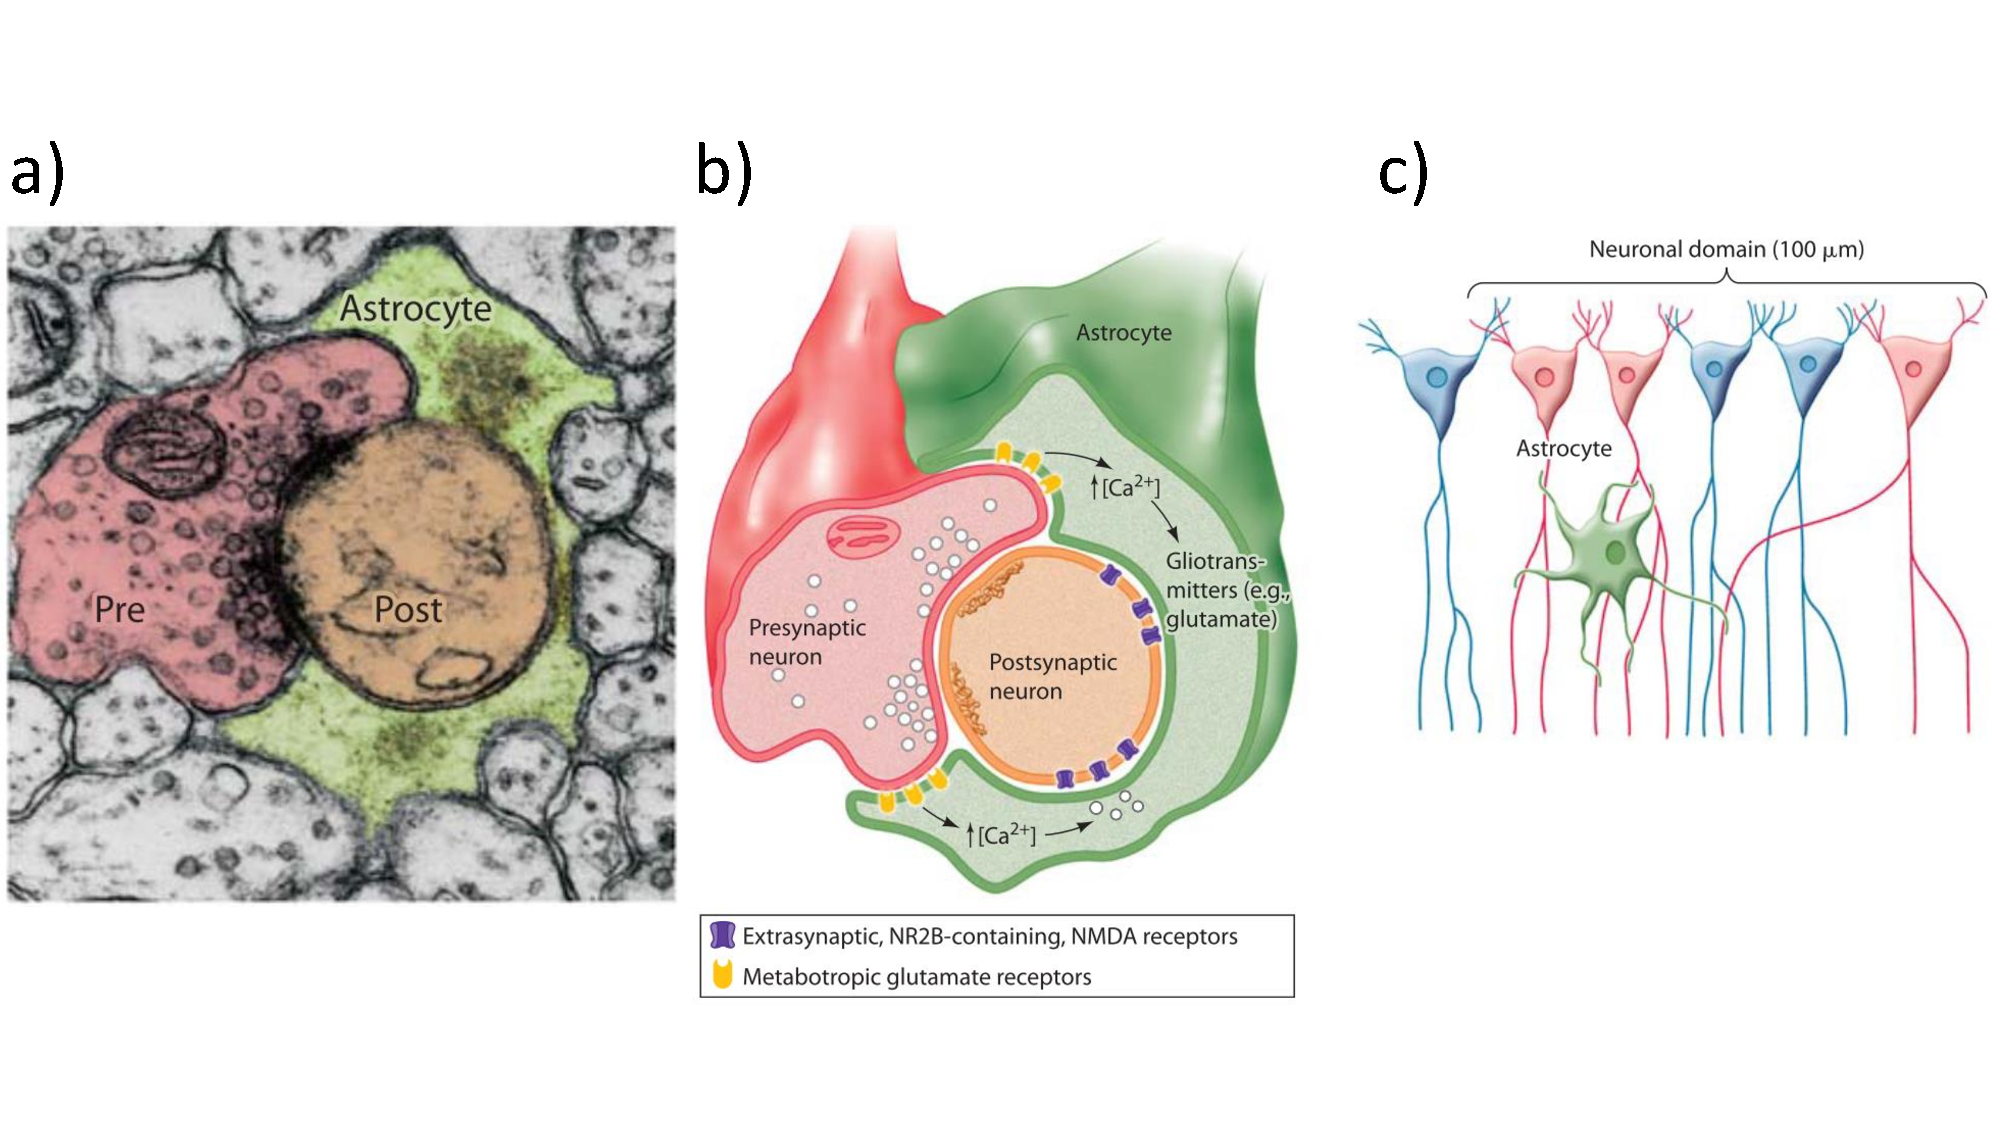
\includegraphics[trim={0 60 0 70},clip,width=\textwidth]{Figures/Chapter1/intro_fig_astro_neuron_modulation.pdf}
    \caption[The tripartite synapse model]{\textbf{The tripartite synapse model.} 
    A) Electron microscopy shows the tripartite nature of synaptic structures with astrocytic processes (green) associated with pre- and postsynaptic terminals. 
    Adapted from \cite{mariotti2018}. 
    B) Schematic representation of A), where, in the hippocampus, metabotropic receptors in the plasma membrane of the nearby astrocytic processes are activated by glutamate released from the presynaptic Schaffer collateral terminals.
    As a result of this activation, intracellular $Ca^{2+}$ increases in the astrocytes, which, in turn, leads to the release of glutamate from glial cells through the fusion of tetanus toxin-sensitive vesicles. 
    Astrocytic glutamate selectively acts on extrasynaptic NR2B-containing NMDA receptors to trigger slow inward currents (SICs) in pyramidal CA1 neurons. 
    C) Schematic representation of the mechanisms by which a single astrocyte (green cell) can lead to neuronal synchronization of local clusters of neurons or neuronal domains (red cells) through glutamate release. 
    B) and C) are adapted from \cite{fellin2006}}
    \label{fig:chap1:astro_neuro_modulation}
\end{figure}

Gliotransmission has been observed to modulate \textbf{synaptic plasticity}.
For example, astrocytes have been shown to be involved in heterosynaptic depression in the hippocampus [\cite{pascual2005}; \cite{serrano2006gabaergic}; \cite{andersson2007}; \cite{chen2013heterosynaptic}].
Moreover, clamping $Ca^{2+}$ in individual CA1 astrocytes blocks LTP induction at nearby excitatory synapses by decreasing the occupancy of NMDAR coagonist sites [\cite{henneberger2010}].
Exogenous D-serine or glycine application reverse this effect. 
However, the release of D-serine from astrocytes is controversial, and a novel hypothesis is that astrocytes release l-serine rather than D-serine and shuttle it to neurons for D-serine synthesis [\cite{wolosker2016rise}]. 
Astrocytes can also modulate synaptic depression. 
$Ca^{2+}$ clamping in rat barrel cortex astrocytes during development showed impaired t-LTD [\cite{min2012astrocyte}].
Moreover, simultaneously stimulating an astrocyte with depolarizing pulses and afferent fibers resulted in LTD [\cite{min2012astrocyte}].

As described above, a large amount of data supports the view that astrocytes are crucial modulators of synapses and that their activity can regulate synaptic transmissions and plasticity. 
The next obvious question is whether astrocytes can modulate neuronal network activity, brain rhythmogenesis in vivo, and behavior. 
The development of mouse models of impaired gliotransmission and new more precise genetic tools for cell-specific manipulation offered the opportunity to test these hypotheses. 
By using extracellular and patch-clamp recordings in anesthetized animals, Fellin et al. showed that the selective expression of a dominant-negative form of synaptobrevin 2 in astrocytes to inhibit gliotransmission [\cite{pascual2005}; \cite{zhang2004}] results in decreased slow oscillations in the somatosensory cortex [\cite{fellin2009endogenous}]. 
The decreased slow oscillation activity is due to the astrocytic modulation of cortical synapses at least at two different sites. 
First, there is a loss of the tonic level of extracellular adenosine activating A1 receptors, and second there is decreased function of neuronal NMDA receptors. 
Alterations in astrocytic calcium dynamics inhibit slow wave activity, showing the fine causal interplay between both types of cells during brain oscillations [\cite{szabo2017extensive}].
Interestingly, it has been recently proposed that astrocytes might play a role in the regulation of neuronal membrane potential oscillations at a wide range of frequencies [\cite{bellot2018astrocytic}].
Indeed, the blockade of $K^+$ uptake or astrocytic connectivity enhances the network excitability and forms high-power network oscillations.
This could be due to changes in the oscillatory behavior of individual neurons, which is a well-known effect in the system dynamics field.
More recently, astrocytes have been shown to modulate behavior. 
For example, astrocytes control sleep behavior [\cite{halassa2009astrocytic}], enhance performance in memory tasks [\cite{adamsky2018astrocytic}], and sustain goal-directed behavior [\cite{mederos2020gabaergic}].

Overall, the data presented in this section point to astrocytes as key regulators of neuronal function, from individual synapses, to network activity and behavior. 

% =========================================================== %
%        Subsection: Astrocytes accumulate evidence           %
% =========================================================== %
\subsection{Astrocytes accumulate evidence}
\label{chap1:sec:2:subsec4:astro_evidence}
In the previous sections, we discussed how astrocytes are involved in the way in which neurons process information, focusing mainly on the mechanisms by which these interactions may take place.
However, to further explore the hypothesis that the brain works through the concerted action of an extended network of both neurons and glial cells, the next question is whether astrocytes or astrocytic networks process information themselves and, if so, how. 

Some very recent findings, started addressing this question [\cite{yumu2019glia}; \cite{mederos2020gabaergic}; \cite{kang2020activation}]. Here we will focus on one of them [\cite{yumu2019glia}].  
The Misha Ahrens group studied the interplay of astrocytic and neuronal networks during swimming adaptation strategies and information integration in larval zebra fish [\cite{yumu2019glia}]. 
In this task, animals were exposed to a virtual reality environment where visual feedback was decoupled from motor actions so that swim behavior failed to trigger the expected visual flow. 
The animals, after becoming aware of the futility of their efforts, became passive and stopped moving, trying again a few seconds later (Figure \ref{fig:chap1:astro_evidence}A). 
When the animals switched from the active to the passive behavioral state, the whole-brain average neuronal activity decreased, while the glial activity increased. 
In this case, activity refers to $Ca^{2+}$ transients that started seconds before and peaked after passivity onset (Figure \ref{fig:chap1:astro_evidence}B). 

\begin{figure}
    \centering
    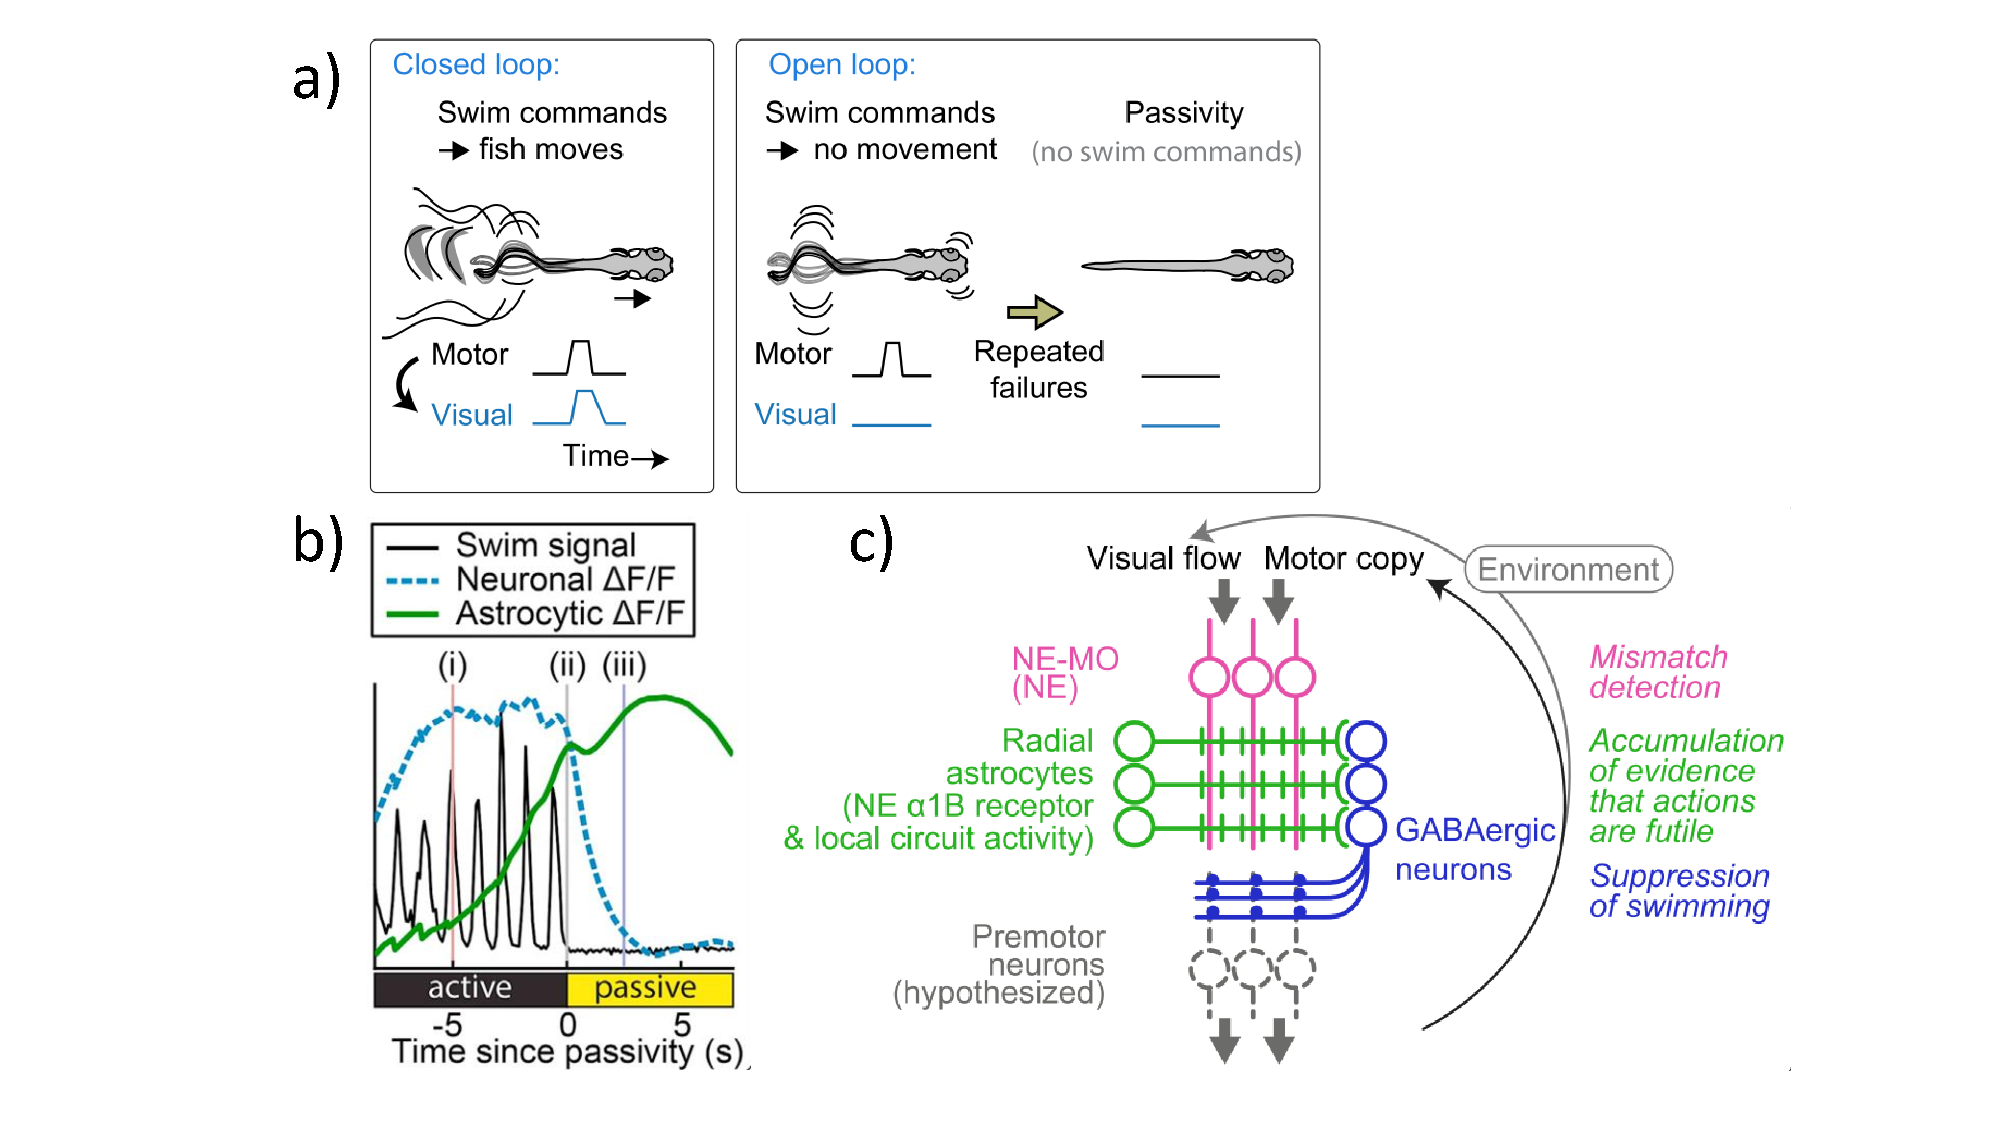
\includegraphics[trim={140 0 100 0},clip,width=\textwidth]{Figures/Chapter1/intro_fig_astro_evidence.pdf}
    \caption[Astrocytes in zebrafish accumulate evidence]{\textbf{Astrocytes in zebrafish accumulate evidence.} 
    A) Locomotion in closed loop versus open loop. 
    Zebrafish entered a passive behavioral state after repeated swim failures. 
    B) Averaged neuronal and glial signals near passivity onset for one representative animal.
    The average neuronal calcium activity decayed after passivity onset, while the glial calcium activity increased before passivity onset and peaked soon after. 
    C) Schematic representation of the circuit hypothesized by the authors: mismatch signals computed from visual and motor efferent inputs are represented by specific neuronal circuits. 
    Noradrenergic axons excite glial processes belonging to astrocytes that integrate mismatch signals and suppress swimming through the activity of downstream GABAergic neurons. 
    Adapted from \cite{mu2019}.}
    \label{fig:chap1:astro_evidence}
\end{figure}
The availability of chemical, optical, and genetic tools allows interventional approaches that can test the causal role of astrocytes in this process. 
On one hand, the reduction of astrocytic $Ca^{2+}$ activity by two-photon laser ablation of glial cells or blocking the inositol 1,4,5-trisphosphate receptor to reduce Ca2+ release from intracellular stores led to a reduction in  futility-induced passivity. 
On the other hand, using a chemogenetic approach to increase intracellular $Ca^{2+}$ in glia led to an increase in the time spent in the passive state. 
This effect was temporally tuned as shown by optogenetic activation of radial astrocytes (using either CoChR or Opto-a1-AR), suggesting that astrocytic $Ca^{2+}$ signals are necessary and sufficient for the expression of this behavior. 

Interestingly, the way astrocytes exert this effect on behavior is achieved through finely tuned interplay between neuronal and astrocytic networks. 
More precisely, during futility-induced passivity, signals from noradrenergic (NE) neurons together with local circuit activity triggered glial responses, as proven by optogenetically activating NE neurons, showing that astrocytes integrate both behavioral information and NE signals.
Astrocytes, in turn, activated GABAergic neurons that would most likely suppress swimming. 

Importantly, through a series of complex but very elegant probabilistic experiments, the group demonstrated that NE neuron signals encode sensory-motor mismatch signals.
Signals are transmitted to astrocytes, which in turn \textit{accumulate evidence} that actions are futile and control swimming behavior through GABAercig neurons (Figure \ref{fig:chap1:astro_evidence}C). 

This study is a beautiful example of the complexity of astrocytic physiology, and it commbines several of the characteristics of astrocytes discussed in the previous sections in an orchestrated mechanism and behaviorally relevant context. 
This study shows how astrocytes are involved in network state changes, integrate neuronal activity, modulate downstream circuits, influence behavior and, importantly, process information in multiple ways.  

% ================================================================ %
% Section: Astrocytes encode spatial information in Ca2+ activity  %
% ================================================================ %
\section{Astrocytes encode spatial information in their $Ca^{2+}$ dynamics}
\label{chap1:sec3:astro_spat_info}
In the following sections, we introduce recent unpublished work from my supervisor's laboratory in collaboration with Jacopo Bonato and Stefano Panzeri. These results significantly contributed to the conceptual development of the work presented in this thesis.
As we previously introduced, astrocytes are involved in the processing of information in the brain, both by encoding specific aspects of behavioral variables and their relations with the environment and by interacting with neuronal networks. 
Astrocytes and their interactions with neurons have been extensively studied in the hippocampus [\cite{perea2007}; \cite{pascual2005}; \cite{serrano2006gabaergic}; \cite{andersson2007}; \cite{chen2013heterosynaptic}; \cite{covelo2018}; \cite{fellin2004neuronal}; \cite{fellin2006purinergic}]. 
However as discussed in the first part of this introduction, one of the most interesting and thoroughly studied functions of hippocampal networks is the encoding of spatial information and the building of a cognitive map for spatial navigation.
The questions of whether navigational information is encoded exclusively in neuronal cells or whether it involves the extended brain network comprising glial cells as well as neurons and whether hippocampal astrocytes intervene in, alter, or modulate spatial information encoding in neurons are still open. 
In my mentor's laboratory, we have started tackling these questions. 
Given that the experimental results that we obtained required precise quantification of spatial information, in the next section, I will introduce information theory and its main statements.  

% =========================================================== %
%              Subsection: Information Theory                 %
% =========================================================== %
\subsection{Information Theory}
\label{chap1:sec:3:subsec1:information_theory}
C. E. Shannon critically contributed to the development of Information theory. 
In his landmark paper \textit{A Mathematical Theory of Communication} [\cite{shannon1948}], Shannon developed a mathematical formalism of communications, considering the coding and decoding problem of information in noisy channels.
This theory extended to many fields with several practical and theoretical applications-notably, modern computation, quantum mechanics, quantum computation, and neuroscience.
There are several ways of approaching the notion of information, as in Shannon's theory, and here, we will expose a modified version of the one exposed in his original paper.
We will start by initially taking his approach because it relates information to probability distributions in an intuitive way. 
However, it's useful to keep the objective in mind, which is what we are trying to use information theory to address. 
The question that we'll try to answer is as follows: if we look at neuronal activity, how much information do we gain from a certain behavioral variable (for example, in the context of spatial navigation, the position of the animal)? 

Let us first try to formalize the problem-neurons can be in several states, depending on how we describe them. 
We can think of a neuron as a variable with two states, either firing or not, or with a continuum of states, such as all the possible values of its membrane potential or of the calcium concentration inside the cell.
Let us then consider, in a general way, that each state of the neuron has a certain probability, namely, state $x$ has probability $p_x$ of occurring.
When we observe a neuron we gain information about its state, e.g., whether or not the neuron is firing. 
However, before measuring it, we can ask the question of \textbf{how uncertain we are about the state of the neuron if we know the set of probabilities $\{p(x)\}$}.
This is equivalent to asking the question concerning \textit{how much} information we will gain when we learn the state of the neuron. 
In this example, we use the state of a neuron, but the approach can be generalized to any probability distribution.
To answer a 'how much' question (either how much uncertainty we have or how much information we gain), we need a quantitative measure. 
Let us call this measure $H$.
There are three reasonable properties that $H$ should have, as follows:
\begin{itemize}
    \item \textbf{$H$ should be a function only of the probabilities}, regardless of the identity of the object to which $H$ refers (e.g., if the object is a cell, then it does not matter whether the cell is a principal neuron, an interneuron, an astrocyte). 
    What is important is that the probabilities of states are the same; therefore we can write $H(p_x)$.
    In addition, \textbf{$H$ should be continuous in $p_x$}.
    \item If all events are equally possible, that is, $p_i=\frac{1}{n}$, with $n$ being the number of states, then \textbf{$H$ should be a monotonically increasing function of $n$}.
    Intuitively, this can be understood as follows: when there are more possible states and all the states are equally possible, there is more uncertainty.
    \item The information gained when two independent events occur with individual probabilities $p$ and $q$ is the sum of the information gained from each event alone.
\end{itemize}
It can be shown [\cite{shannon1948}] that the only $H$ that satisfies all three properties is of the form: 
\begin{equation}
    H=-K \sum_{x=1}^n p_x\ log (p_x)
\end{equation}
where $K$ is a positive constant that determines the choice of units of measure.
This definition of $H$ falls under the name of \textbf{entropy}. 
We select the logarithm to be in base $2$ (all logarithms in this thesis will be in base $2$ unless otherwise specified), which is achieved by appropriately selecting the constant $K$, and define the entropy of the probability distribution $p_1,p_2,...,p_n$ of an $n$ state variable as:
\begin{equation}
\label{eqn:entropy}
    H=- \sum_{x=1}^n p_x\ log_2 (p_x)
\end{equation}
This definition is intuitive and has the advantage that it can be used to \textit{quantify the resources needed to store information}. 
It can be shown that Shannon's entropy represents the minimal physical resources required to store the information being produced by a source in such a way that at a later time, the information can be reconstructed.
This result is known as \textit{Shannon’s noiseless coding theorem} [\cite{shannon1948}].

To illustrate some of the properties of $H$, we provide an example. Let us consider a simplified neuron with two possible functional states: firing and not firing. The neuron fires with probability $p$ and is silent with probability $q=1-p$. Its entropy is given by:
\begin{equation}
    H=-(p\ log (p) + (1-p)\ log (1-p))
\end{equation}
We can see the values of $H$ as a function of $p$ in Figure \ref{fig:chap1:info_theory_concepts}A.
If the neuron is always silent and never fires, we have no uncertainty regarding its state, and we gain no information by measuring its state.
Under these conditions, $p=0$, and therefore, $H=0$.
If, on the other hand, the neuron randomly fires half of the time, we have maximal uncertainty about its state before measurement, and therefore, we gain the maximum amount of information after measurement.
Thus, $p=0.5$, and the entropy is $H=1$.
In other words, this means that knowing the state of the neuron gives us $1$ bit of information.
In general, we have $H=0$ if and only if all $p_i=0$ except one, which is $1$. 
The uniform distribution is the probability distribution with the maximum entropy, and in this case, the entropy is the logarithm of the number of states.
That is, $H=log(n)$, and it is maximum if and only if $p_i=\frac{1}{n} \; \forall \ i$.

\begin{figure}
    \centering
    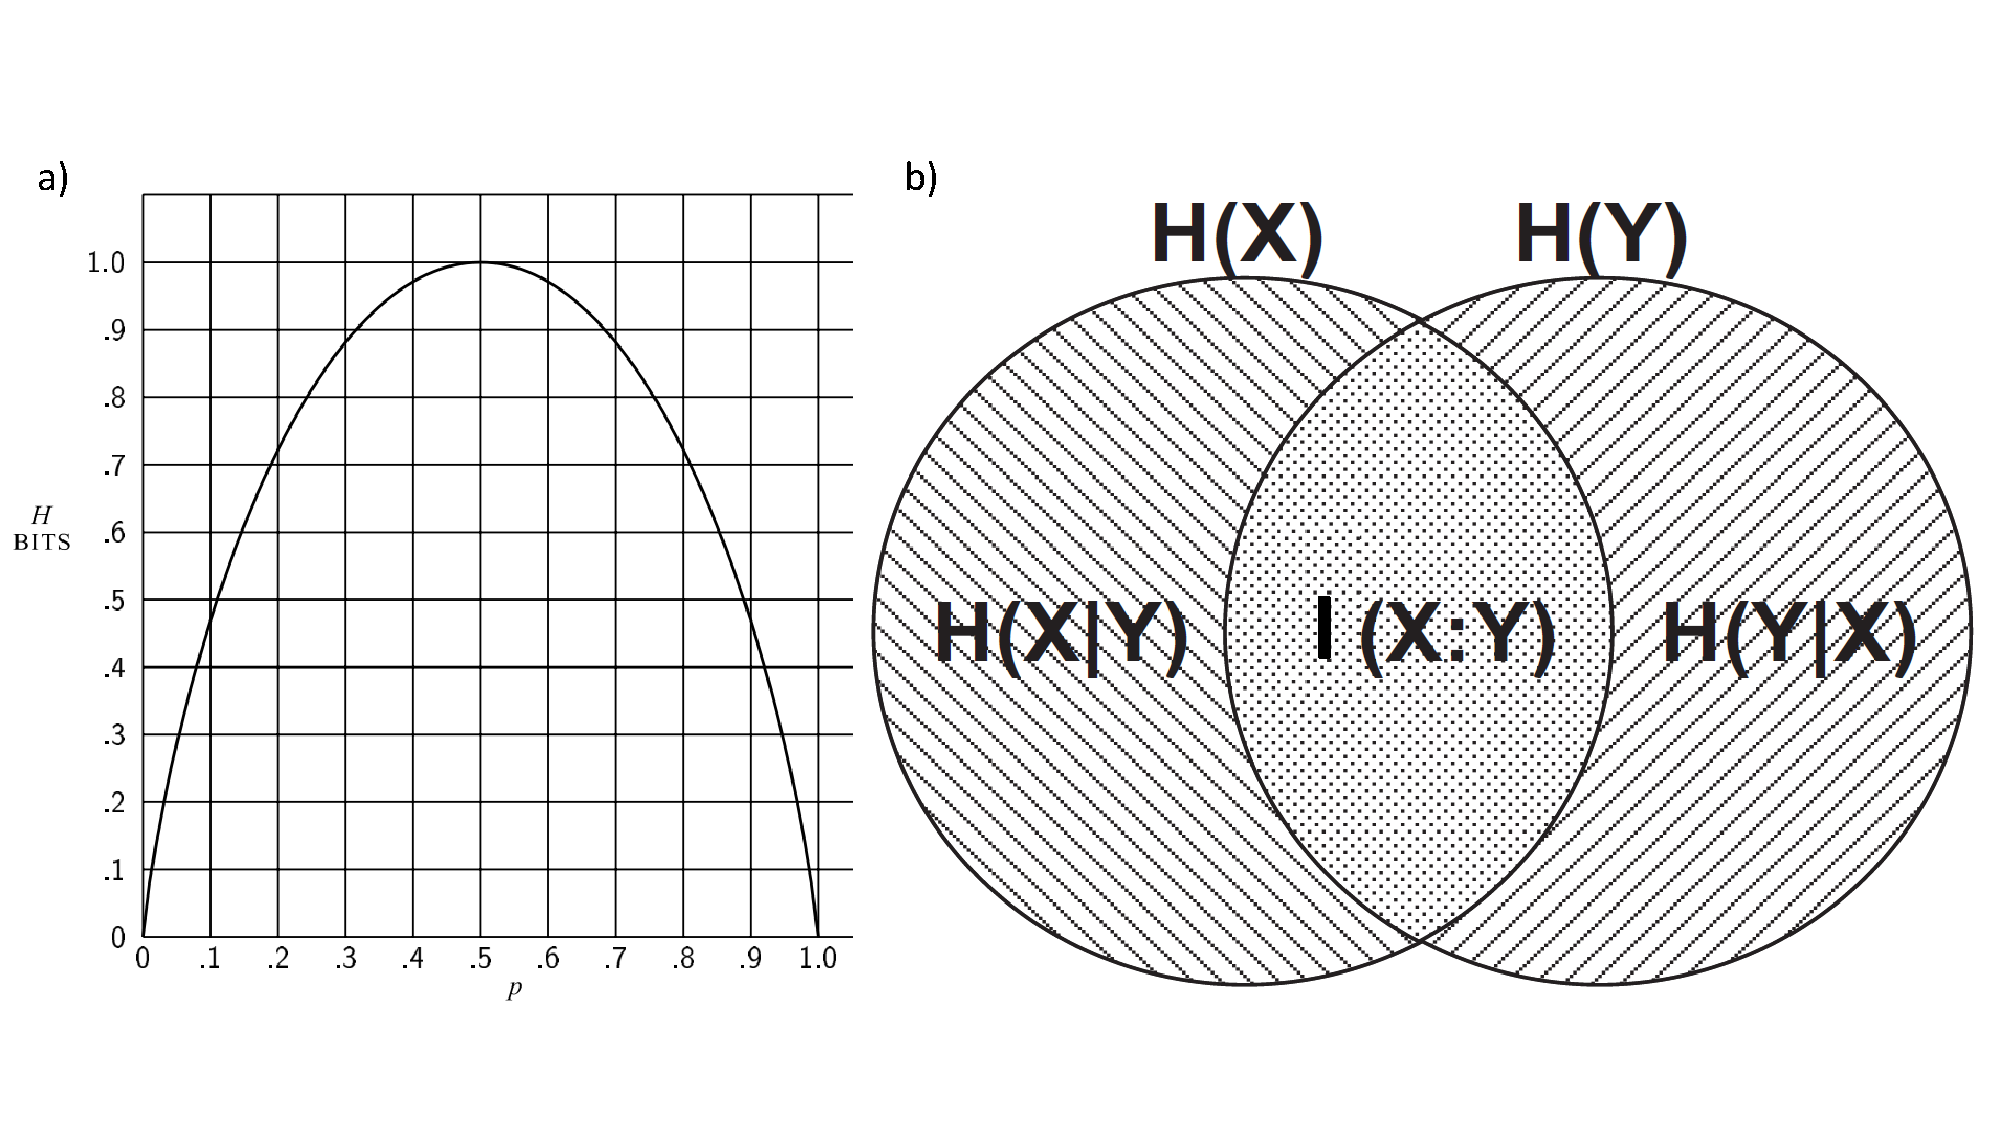
\includegraphics[width=\textwidth]{Figures/Chapter1/intro_fig_info.pdf}
    \caption[Entropy and information theory]{\textbf{Entropy and information theory.} 
    A) Entropy of a binary variable as a function of the probability $p$, adapted from \cite{shannon1948}. 
    B) Schematic entropy and information Venn diagram, adapted from Nielsen and Chuang book, 2010.}
    \label{fig:chap1:info_theory_concepts}
\end{figure}

In addition to $H$, there are other important quantities to define in information theory.
Let us hypothesize that we have another variable, $Y$, with its own states and probability distribution ${p(y)}$, that can represent another neuron or set of neurons, or a behavioral variable such as the position of the animal. 
We define the \textbf{joint entropy} of variables $X$ and $Y$ as
\begin{equation}
\label{eqn:jointentropy}
    H(X,Y)\equiv-\sum_{x,y}p(x,y)\ log(p(x,y)) 
\end{equation}
The joint entropy measures the total uncertainty about the pair $(X,Y)$.
A third important quantity applies to the following situation: suppose that we learn the value of $Y$, meaning that we gain $H(Y)$ bits of information about the pair $(X,Y)$.
How much uncertainty remains about the pair $(X,Y)$? 
Or in other words, how uncertain are we about $X$, given that we know the value of $Y$?
This quantity is called the \textit{entropy of $X$ conditioned on knowing $Y$} and is defined as:
\begin{equation}
\label{eqn:condentropy}
    H(X\ |\ Y) \equiv H(X,Y)-H(Y)
\end{equation}
With the definition provided above, we now have everything we need to define the quantity that addresses our initial question, i.e., if we look at neuronal activity, how much information do we gain from a certain behavioral variable (for example, the position of the animal)? 
Alternatively, how much information is shared between neuronal activity and the behavioral variable?
We can formalize this situation as follows.
Let us consider two variables $X$ and $Y$, and suppose that we add the information content of $X$, $H(X)$ to that of $Y$, $H(Y)$.
If there is information shared between the two variables, then we will count it twice, and information that is not common will be counted only once. 
Therefore, if we subtract from the sum of $H(X)$ and $H(Y)$, the total amount of information of the pair, which is nothing but the joint entropy $H(X,Y)$, what remains is the common or \underline{\textbf{mutual information}} of $X$ and $Y$:
\begin{equation}
\label{eqn:mutualinfo1}
    I(X:Y)\equiv H(X)+H(Y)-H(X,Y)
\end{equation}

In the last paragraph, we have been using \textit{information} and entropy as somewhat interchangeable concepts.
This is because, as we said at the beginning of this section, entropy quantifies the amount of uncertainty about a variable before knowing its state or, equivalently, how much \textit{information} we gain about that variable when we measure its state.
However, we could arrive, at the expression for mutual information in a slightly different but equivalent way.
As we saw before \textit{conditional entropy} $H(X\ |\ Y)$ represents the uncertainty that remains in $X$ given that we learned the value of $Y$.
Thus, the complement of the uncertainty that remains is the \textit{information that we gained} about $X$ by knowing $Y$. 
Formally, we can then define \textit{mutual information} as: 
\begin{equation}
\label{eqn:mutualinfo2}
    I(X:Y)\equiv H(X) - H(X\ |\ Y)
\end{equation}
The equivalency of expressions \ref{eqn:mutualinfo1} and \ref{eqn:mutualinfo2} is trivially shown simply by replacing \ref{eqn:condentropy} in \ref{eqn:mutualinfo1}.
A useful way of visualizing the various definitions of entropic quantities is the 'entropy Venn diagram' shown in figure \ref{fig:chap1:info_theory_concepts}B. 

Information theory has been widely applied in neuroscience, starting from the works of Richmond and Optican in 1990 [\cite{richmond1990temporalI}; \cite{richmond1990temporalII}] on the primate visual cortex and the Skaggs formula for spiking activity in 1992 [\cite{skaggs1992information}].
There are several reasons for the success and usefulness of information theory approaches for studying the brain.
First, information theory is model-independent in the sense that there is no a priori model of the interaction between the variables of the system under study.
This does not mean that information theory is \textit{assumptions}-free. 
Rather, there are several assumptions about the data that need to be made. 
For example, it is required to assume the data to be stationary, i.e., if a neuron encodes information about a behavioral variable at the beginning of the experiment, it will do so at the end.     
Second, because of its probabilistic nature, information theory is applicable regardless of the data type, meaning that we can use it if one of the variables is represented by a binary signal, as in the case of spikes in a neuron, or if it is a continuous variable, as in the speed of an animal in $cm/s$.
Third, information theory can uncover nonlinear relations between variables.
Finally, all the quantities presented so far are easily scalable to many variables and are therefore applicable to many neurons or combinations of a neuron and several behavioral variables.

Information theory also has limitations when applied to neuroscience. 
For example, information theory would require knowledge of the true probability distributions of considered variables, but this information is not available in the experimental neuroscience setting.
Most of the time, experimentally measured probability distributions are only good approximations of true distributions.
The bias implied by using empirical probability distributions has been extensively studied, and several alternatives for correcting such bias have been proposed [\cite{panzeri2007}; \cite{panzeri1996}; \cite{treves1995}].

Information theory approaches have been traditionally used for studying spiking trains and therefore electrophysiological data [\cite{skaggs1992information}].
However, as we said before, this approach can be used regardless of the nature of the data types, and more recently, it has been used for analyzing the information content and correlations in calcium activity as recorded by 2-photon imaging [\cite{shuman2020breakdown}; \cite{stefanini2020distributed}; \cite{rubin2015hippocampal}; \cite{sheintuch2017tracking}; \cite{runyan2017distinct}].
% =========================================================== %
%        Subsection: Astrocytes and information               %
% =========================================================== %
\subsection{Astrocytes and spatial information}
\label{chap1:sec:3:subsec2:astro_info}
In the context of information theory and spatial navigation, the first outstanding question is whether astrocytes encode spatial information about the position of the animal in the dynamics of intracellular calcium signals.
Here, we will summarize recent unpublished data from my mentor's laboratory that contribute to answering this question.
To test this hypothesis, mice were trained to run head-fixed in a virtual reality corridor (Figure \ref{fig:chap1:seba_1}A) [Gauthier and Tank 2018].
Astrocyte-specific expression of the genetically encoded calcium indicator GCaMP6f [\cite{chen2013}; \cite{haustein2014conditions}] was used together with two-photon functional imaging to capture the subcellular calcium dynamics of hippocampal CA1 astrocytes (Figure \ref{fig:chap1:seba_1}C). 
It was found that a fraction of subcellular regions carried significant information about the spatial position of the animal in the virtual track (Figure \ref{fig:chap1:seba_1}B,D).
In this context, \textit{significant amount of information} is related to how the mutual information value compares to surrogate distributions of MI values built by temporally shuffling the data (see methods for details). 
The distribution of response field positions covered the entire length of the virtual corridor (Figure \ref{fig:chap1:seba_1}D), suggesting a full map of the environment produced by astrocytes, which was parallel (or complementary) to that of the neuronal network.
Similar to neurons, when exposed to a bidirectional environment, astrocytic ROIs showed significant direction selective spatial modulation in their response field.

\begin{figure}
    \centering
    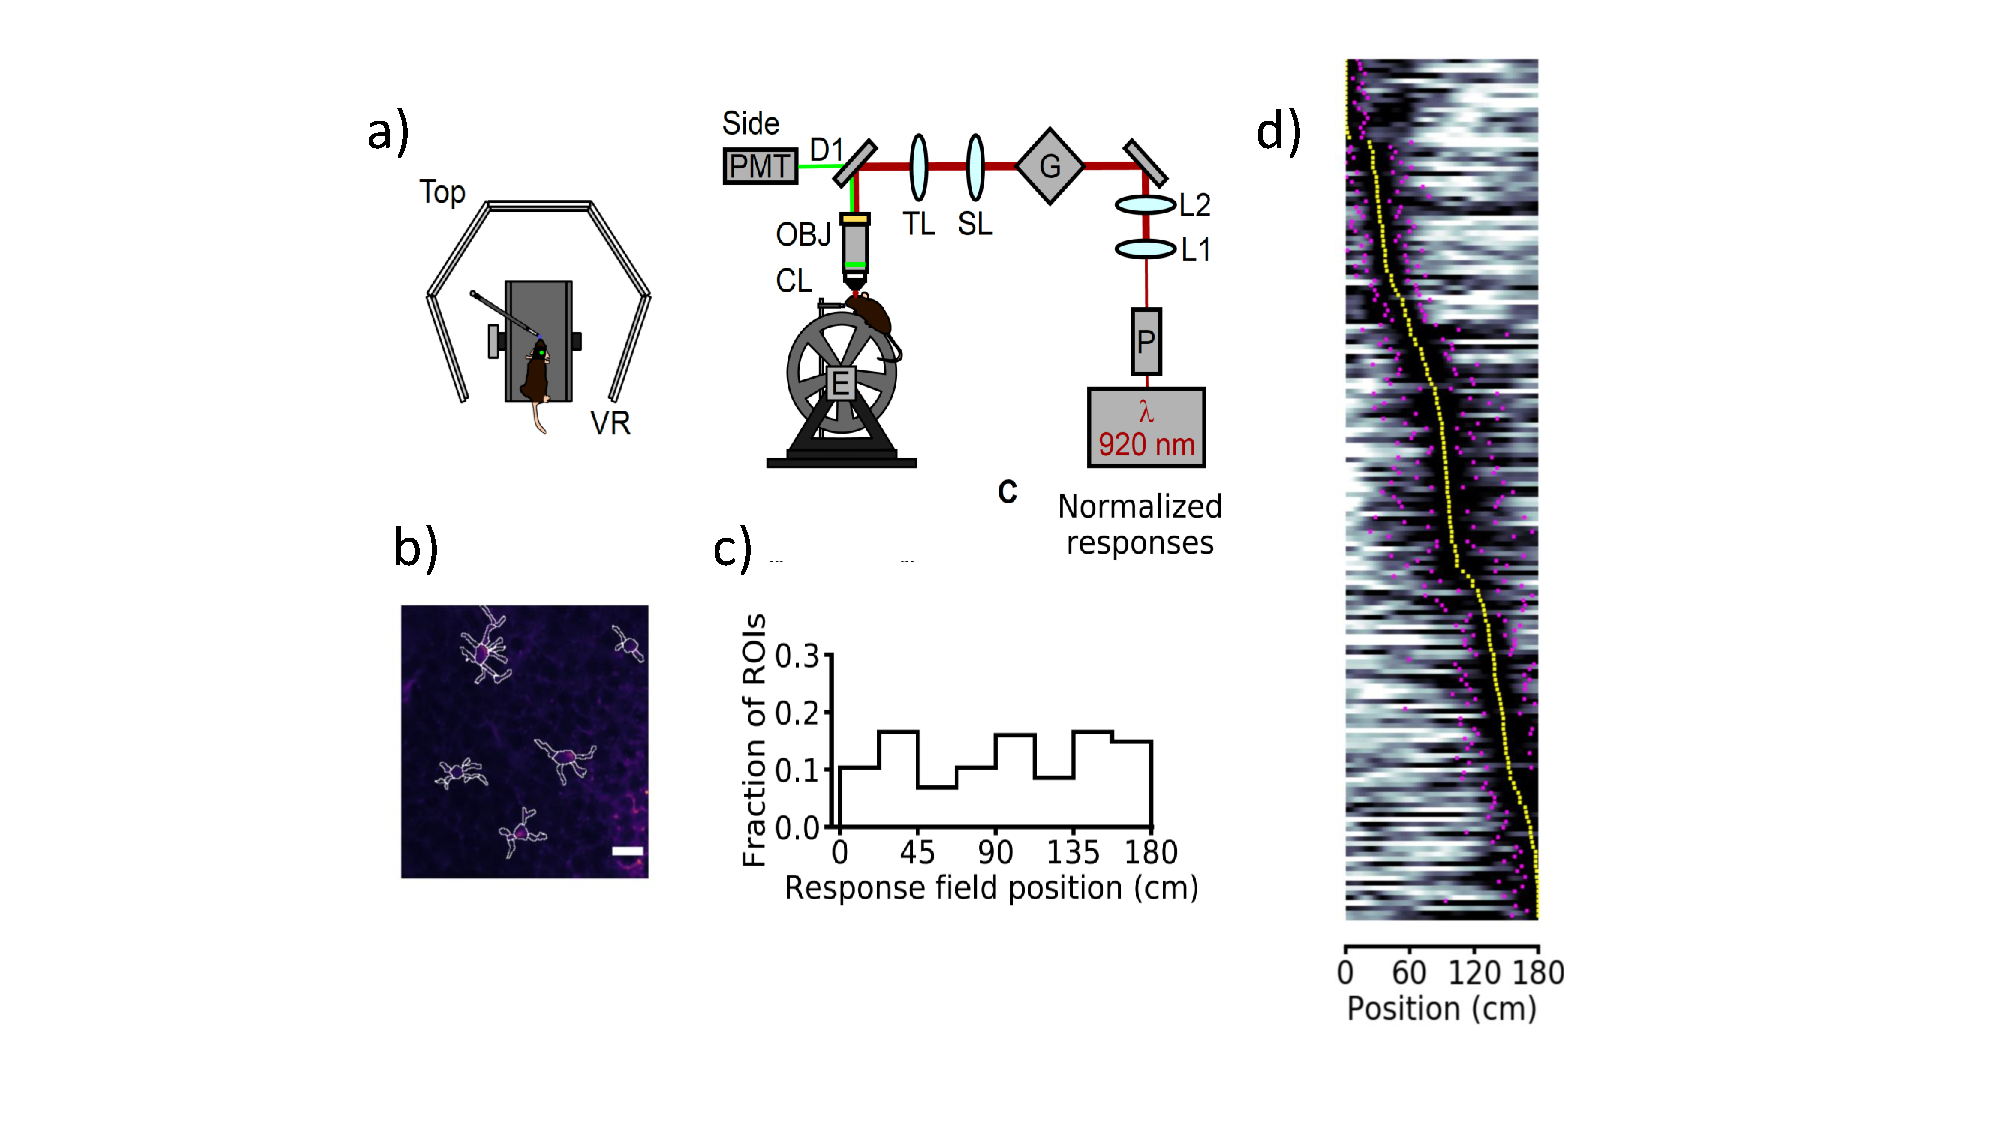
\includegraphics[trim={150 50 200 0},clip,width=\textwidth]{Figures/Chapter1/intro_fig_seba_1.pdf}
    \caption[Calcium dynamics in astrocyte networks in the hippocampus encode spatial information]{\textbf{Calcium dynamics in astrocyte networks in the hippocampus encode spatial information.} 
    A) Schematics of the experimental setup. 
    Head-restrained mice run on a treadmill while navigating a virtual corridor. 
    B) Normalized astrocytic calcium responses as a function of position for astrocytic ROIs that contain significant amount of spatial information. 
    Yellow dots indicate the center position of the response field, and magenta dots indicate its width (vertical scale: 50 ROIs)
    C) Median projection of GCaMP6f-labeled astrocytes in the CA1 pyramidal layer. 
    Segmented ROIs are shown in white; scale bar, 20 $\mu m$. 
    D) Distribution of response field positions. 
    Adapted from Curreli, Bonato, Romanzi, Panzeri and Fellin, submitted.
    }
    \label{fig:chap1:seba_1}
\end{figure}
It was found that both cell bodies and processes encoded spatial information and that a similar fraction of somas and processes were modulated by the spatial position of the animal (Figure \ref{fig:chap1:seba_2}A,B).
The preferred field position of astrocytes was not entirely random.
This was observed first because the correlation between the calcium activity of pairs of informative ROIs decreased as a function of the pair distance (Figure \ref{fig:chap1:seba_2}D).
Second, the difference between the field positions of the two informative ROIs in a given pair increased as a function of the pair distance within $0-40 \mu m$ and reached a constant value, indicating that informative calcium signals were coordinated across cells (Figure \ref{fig:chap1:seba_2}C).
Similarly, when looking at the single cell-level, the difference between the field position of an informative process and the corresponding somas increased as a function of the process distance from the soma (Figure \ref{fig:chap1:seba_2}E), demonstrating that spatial information is differentially encoded in topologically distinct locations of the same astrocyte. 
Overall, these results demonstrate that astrocytes encode spatial information in the hippocampus during virtual navigation, and that a complete map (at least in a unidimensional virtual track) could be encoded in the astrocytic network (meaning that the place fields of all astrocytes observed spanned the whole length of the virtual corridor).
\begin{figure}[h]
    \centering
    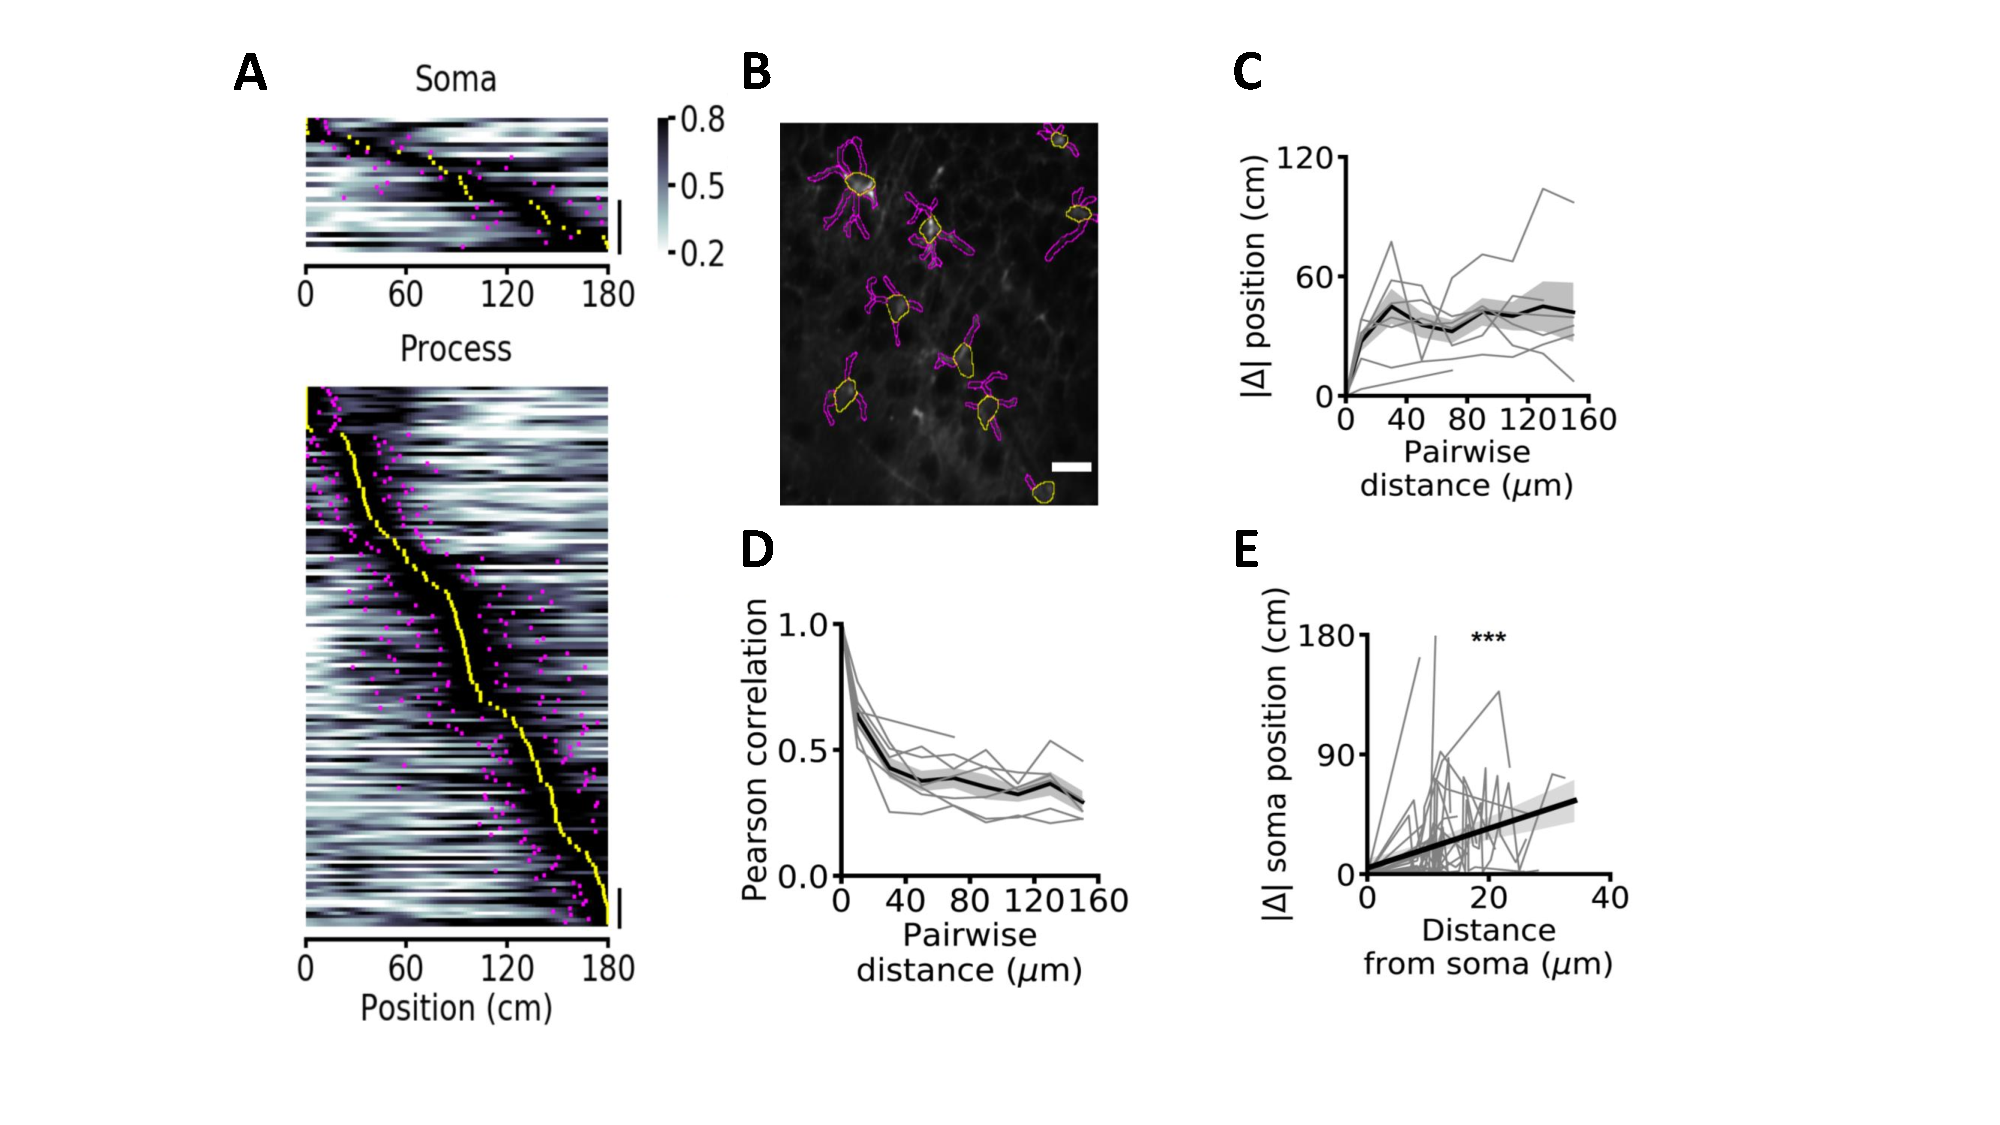
\includegraphics[trim={110 40 130 0},clip,width=\textwidth]{Figures/Chapter1/intro_fig_seba_2.pdf}
    \caption[Spatial information is encoded differentially in astrocyte somas and processes]{\textbf{Spatial information is encoded differentially in astrocyte somas and processes.} 
    A) Normalized astrocytic calcium responses as in \ref{fig:chap1:seba_1}B for ROIs corresponding to somas (top) and processes (bottom) (vertical scale: 10 ROIs). 
    B) Median projection of a t-series displaying GCAMP6f-labeled astrocytes in the CA1 pyramidal layer. ROIs are separated into somas (yellow) and processes (magenta). 
    Pairwise Pearson’s correlation (D) and difference between response field positions (C) for pairs of astrocytic ROIs across the whole FOV as a function of the ROI pairwise distance. 
    E) Difference in the response field position of a process with respect to the field position of the corresponding soma as a function of the process distance from the cell soma.
    Adapted from Curreli, Bonato, Romanzi, Panzeri and Fellin, submitted.}
    \label{fig:chap1:seba_2}
\end{figure}
% =========================================================== %
%             Subsection: Decoding of position                %
% =========================================================== %
\subsection{Decoding of position}
\label{chap1:sec:3:subsec3:position_decoding}
Is it possible to decode the animal's position based on the calcium dynamics of astrocytes during navigation in the virtual corridor? 
To answer this question, a support vector machine (SVM) was trained to solve the classification problem of decoding the mouse's position using single-trial astrocytic calcium signals according to a set of discrete locations. 
% The decoder accuracy, which represented how many times the decoder correctly classified the position of the mouse, was significantly above chance level, regardless of how many discrete locations were available in the space domain (Figure \ref{fig:chap1:seba_3}A). 
% This is important because it means that a downstream neuron (or network) would be able to decode animal's position by integrating astrocytic calcium transients information, suggesting the potential behavioral relevance of this process. 
% The decoding accuracy decreased with increasing spatial granularity but remained significantly above chance for all spatial granularity values used (Figure \ref{fig:chap1:seba_3}B).  
The decoder decoded spatial information was significantly above chance level, regardless of how many discrete locations were available in the space domain (Figure \ref{fig:chap1:seba_3}A).
Disrupting temporal coupling within astrocytic population vectors while preserving single-ROI activity patterns, which was achieved by shuffling spatial information in the data while preserving the temporal features of the calcium signals, consistently decreased decoded spatial information (Figure \ref{fig:chap1:seba_3}A).
This is important because it means that a downstream neuron (or network) would be able to decode animal's position by integrating astrocytic calcium transients information, suggesting the potential behavioral relevance of this process. 
Misclassifications were more likely to occur among nearby locations across all granularity conditions (Figure \ref{fig:chap1:seba_3}B), meaning that decoder errors are not uniformly distributed and suggesting that errors made are \textit{reasonable errors} and not random misclassifications.
\begin{figure}[h]
    \centering
    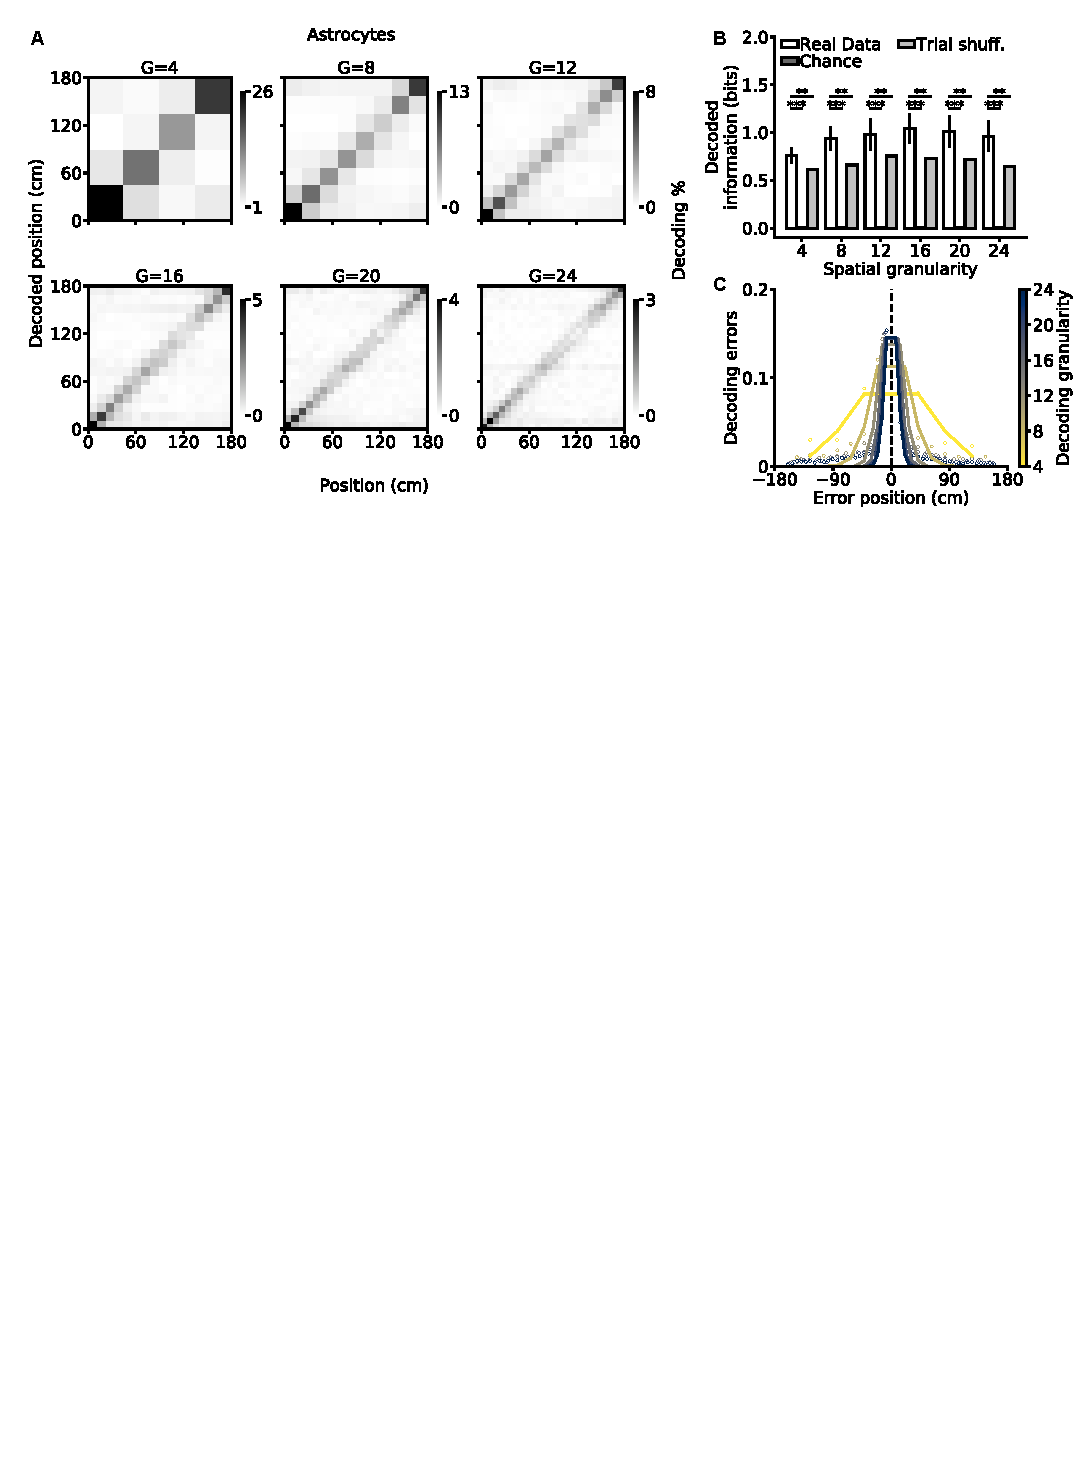
\includegraphics[trim={0 80 0 0}, clip, width=\textwidth]{Figures/Chapter1/intro_fig_seba_3.pdf}
    \caption[Animal spatial location can be efficiently decoded from astrocytic calcium signals]{\textbf{Animal spatial location can be efficiently decoded from astrocytic calcium signals.} 
    % A) The decoding accuracy as a function of the decoding spatial granularity in real (black line) and shuffled (gray line) data. 
    % B) Amount of information in bits retrieved by the SVM decoder as a function of the granularity. 
    %C) The decoding error as a function of the error position within a confusion matrix. The decoding granularity is represented as different lines.}
    A) Amount of information in bits retrieved by the SVM decoder as a function of the granularity on real (white), chance (dark gray), and trial shuffled (grey) data (see methods). Trial-shuffling disrupts temporal coupling within astrocytic population vectors, while single-ROI activity patterns are preserved.
    B) The decoding error as a function of the error position within a confusion matrix. The decoding granularity is represented as different lines.
    Adapted from Curreli, Bonato, Romanzi, Panzeri and Fellin, submitted.} 
    \label{fig:chap1:seba_3}
\end{figure}


% =========================================================== %
%                    Subsection: Page Margin                  %
% =========================================================== %
% \subsection{Page Margin}
% \label{chap1:sec:2:subsec1:page_margin}
% The format of page size and margin is defined in ``main.tex'' file \textbf{Line 63-71}. The page margin of the current version template is \uline{Left: 35mm, Right: 36mm (a4paper).} Users can change the page margin by adjusting the corresponding settings. There is no stipulation for the top and bottom margins, but the booklet recommend that both of them should be 25mm, which is adopted in this template. 


% =========================================================== %
%          Subsection: Font, Alignment, Line Spacing          %
% =========================================================== %
% \subsection{Font, Alignment, Line Spacing}
% Ordinarily, there is no restrict stipulation for the font family, font size, alignment, and line spacing. All of these are a matter of personal preference. This template uses \textit{10pt} font size, \textit{Fully Justified} alignment style and \textit{One and A Half} line spacing. Users can adjust the settings in \textbf{Line 19-33} of the ``main.tex'' file to change the typeset.


% =========================================================== %
%                      Subsection: Contents                   %
% =========================================================== %
% \subsection{Contents}
% The contents of this template can be subdivided into three parts --- the front matter, the text and the back matter, which strictly follows the stipulations of the official booklet (Page 17). \tabref{chap1:longtable:checking_list} indicates the what contents are required in the submitted thesis and what contents are optional. The column ``Required'' denotes that 
% \begin{center}
% \begin{longtable}{|l|c|c|}
% \caption{Checking list indicating the contents should be included in the thesis.}\label{chap1:longtable:checking_list}\\
% \hline
% \textbf{The Front Matter} & Required     &  Include $\checkmark$ \\ \hline \hline
% Abstract                  & Yes          & $\checkmark$         \\
% Title Page                & Yes          & $\checkmark$         \\
% Frontispiece              &              &                      \\
% Dedication                &              & $\checkmark$         \\
% Epigraph                  &              &                      \\
% Declarations              & Yes          & $\checkmark$         \\
% Acknowledgements          &              & $\checkmark$         \\
% Table of Contents         & Yes          & $\checkmark$         \\
% List of Illustrations     &              &                      \\
% List of Figures           &              & $\checkmark$         \\
% List of Tables            &              & $\checkmark$         \\
% List of Algorithm         &              & $\checkmark$         \\
% List of Abbreviations     &              & $\checkmark$         \\
% List of Symbols           &              & $\checkmark$         \\
% Others                    &              &                      \\ \hline \hline
% \textbf{The Text}         & Yes          & $\checkmark$         \\ \hline \hline
% \textbf{The Reference or Back Matter} &    ---    &   ---       \\ \hline \hline
% Glossary                  &              &                      \\
% Appendices                &              &                      \\
% Notes                     &              &                      \\
% Bibliography or Reference List & Yes          &  $\checkmark$   \\
% Index                     &              &                      \\
% \hline
% \end{longtable}
% \end{center}
% This template support most of the contents listed in the figure, including the ``Abstract'', ``Title Page'', ``Declarations'', ``Acknowledgements'', ``List of Publications'', ``Contents'', ``List of Figures'', ``List of Tables'', ``List of Algorithms'', ``List of Abbreviations'', ``List of Symbols'', ``Main Text'', ``Appendices'', and ``Bibliography''. Each part is defined in an independent tex file and the ``main.tex'' file combines all the different parts to form the entire thesis. Therefore, users can easily make the changes by adjusting the corresponding document files.

% In addition to the stipulations of the booklet, this template also provides a beautiful \textbf{cover page}, which is the first two pages of this project. \uline{The cover page is \textbf{not required} by the Graduate School and you'd better remove the cover page when bounding your thesis for submission.}








